\section{The reach of a suction trigger}
How far a crop can dry the soil at the sensor, why the limit exists, how the single constant $\kappa$ is found from experiment E2, and how the closed form is checked.

\subsection{Contribution 1: the reach of a suction trigger}\label{con:s4:1}
\begin{problem}
A farmer on a sandy field installs a matric-potential sensor at 20\,cm and sets the common trigger of 300\,cm. All season the controller never opens the valve, the crop wilts, and the yield equals that of a field that was never irrigated. The sensor works. Why is the trigger never reached, and how dry a trigger can be used on any soil, from its van~Genuchten parameters alone?
\end{problem}
\begin{derivation}
\textbf{(a)} Roots dry a layer only as fast as the soil delivers water to them; the delivery is proportional to the conductivity $K=K_sK_r$ \citep{Gardner1960}. \textbf{(b)} Postulate: the sensor's soil stops drying when the relative conductivity has fallen to one value $\kappa$, the same for all soils, $K_r(\hc)=\kappa$. \textbf{(c)} At the dry end, $K_r\simeq m^2(\alpha h)^{-[2n+\ell(n-1)]}$ (Section~\ref{der:s4:2}). \textbf{(d)} Insert (c) into (b): $m^2(\alpha\hc)^{-E}=\kappa$ with $E=2n+\ell(n-1)$. \textbf{(e)} Divide by $m^2$, raise to $-1/E$, divide by $\alpha$.
\end{derivation}
\begin{keyresult}
\begin{pencil}
{\small\noindent\textbf{How it is derived, line by line}
\[\begin{array}{@{}l@{}}\textbf{1. Postulate (uptake stops at one relative conductivity):}\\[1pt]
\qquad K_r(\hc)=\kappa\\[1pt]
\textbf{2. Dry-end form of Mualem (Section \ref{der:s4:2}):}\\[1pt]
\qquad K_r(h)\simeq m^2(\alpha h)^{-E}\\[1pt]
\textbf{2b. Slope of the dry end:}\\[1pt]
\qquad E=2n+\ell(n-1)\\[1pt]
\textbf{3. Insert 2 into 1:}\\[1pt]
\qquad m^2(\alpha\hc)^{-E}=\kappa\\[1pt]
\textbf{4. Divide by } m^2\textbf{:}\\[1pt]
\qquad (\alpha\hc)^{-E}=\kappa/m^2\\[1pt]
\textbf{5. Raise both sides to } -1/E\textbf{:}\\[1pt]
\qquad \alpha\hc=(m^2/\kappa)^{1/E}\\[1pt]
\textbf{6. Divide by } \alpha\textbf{:}\\[1pt]
\qquad \hc=\alpha^{-1}(m^2/\kappa)^{1/E}
\end{array}\]}
\noindent\textbf{The result, with its parts marked}
\[
\hc\;=\;\underbrace{\frac{1}{\alpha}}_{\circled{1}}\;\Bigl(\underbrace{m^{2}}_{\circled{2}}\Big/\underbrace{\kappa}_{\circled{3}}\Bigr)^{\textstyle\overbrace{1/[\,2n+\ell(n-1)\,]}^{\circled{4}}}
\]
\[
\underbrace{\kappa=3.47\times10^{-10}}_{\circled{5}}\]
\[\underbrace{\text{error on soils left out}\le\text{a factor of }2.3}_{\circled{6}}
\]
\end{pencil}
\end{keyresult}
\begin{pins}
\pin{1}{$1/\alpha$ is the suction at which the soil starts to drain. It only \emph{rescales} the reach: two soils with the same $n$ have reaches in the ratio of their $1/\alpha$. This is why, at equal $n$, a soil that starts draining later (small $\alpha$) can be dried further.}
\pin{2}{$m^2=(1-1/n)^2$ comes from the tail of the Mualem integral. It changes slowly with $n$ (0.035 to 0.39 over the ten soils) and enters under the root of order $E$, so its effect is small; it is kept because it makes the formula exact at the dry end.}
\pin{3}{$\kappa$ is the single constant of the law: the relative conductivity at which the crop can no longer dry the soil at the sensor within a season. It is a property of the crop and its uptake, not of the soil, which is why one value serves ten soils. It was fitted once and tested by leaving soils out.}
\pin{4}{The exponent $1/E$ with $E=2n+\ell(n-1)$ is the heart of the result. $E$ is the slope of $\log K_r$ against $\log h$ at the dry end. In sand ($n=2.68$) $E=6.2$: the conductivity collapses within a narrow band of suction, so the reach is short (199\,cm). In silty clay loam ($n=1.23$) $E=2.6$: the conductivity fades slowly, so the reach is long ($1.3\times10^5$\,cm). The pore-size distribution, through $n$, decides how far a crop can dry a soil.}
\pin{5}{$\kappa=3.47\times10^{-10}$ means the soil at the reach conducts about three billion times less than when saturated; with saturated conductivities of 1 to 700\,cm\,d$^{-1}$ this is far below a millimetre per day, which is why uptake stops there.}
\pin{6}{The law was tested on soils it had not seen: each soil was removed, $\kappa$ refitted on the other nine, and the removed soil predicted. Five predictions fell inside the observed interval and none was off by more than a factor of 2.3. A threshold on absolute conductivity, the obvious alternative, failed (it spans more than three decades).}
\end{pins}


\subsection{Contribution 2: a rule for blind triggers}\label{con:s4:2}
\begin{problem}
Which of the tabulated triggers can be used on which soil, before any season is lost?
\end{problem}
\begin{derivation}
The irrigation of every soil fell to zero between $\htr/\hc=0.5$ and 1 (Fig.~3b of the article). A trigger therefore fires reliably only below half the reach. Compute $\hc$ (Contribution~1), halve it, and compare with the trigger.
\end{derivation}
\begin{keyresult}
\begin{pencil}
{\small\noindent\textbf{How it is derived, line by line}
\[\begin{array}{@{}l@{}}\textbf{1. Observation (Fig.~3b):}\\[1pt]
\qquad \text{irrigation}\to0\ \text{for}\ 0.5\le\htr/\hc\le1\\[1pt]
\textbf{2. Keep a margin below the first value:}\\[1pt]
\qquad \htr/\hc<\tfrac12\\[1pt]
\textbf{3. Multiply by } \hc\textbf{:}\\[1pt]
\qquad \htr<\tfrac12\hc
\end{array}\]}
\noindent\textbf{The result, with its parts marked}
\[\underbrace{\htr}_{\circled{1}}\;<\;\underbrace{\tfrac12}_{\circled{2}}\,\underbrace{\hc(\alpha,n,\ell)}_{\circled{3}}\]
\end{pencil}
\centering\small
\begin{tabular}{lrrl}
\toprule
Soil & $\hc$ (cm) & $\hc/2$ (cm) & 300\,cm trigger\\\midrule
Sand (S03) & 199 & 100 & \circled{4} blind: never fires\\
Loamy sand (S04) & 426 & 213 & \circled{4} blind: never fires\\
Sandy loam (S05) & 1\,618 & 809 & fires\\
Loam (S06) & 9\,209 & 4\,605 & fires\\
Silty clay loam (S10) & 128\,260 & 64\,130 & fires\\\bottomrule
\end{tabular}
\end{keyresult}
\begin{pins}
\pin{1}{The trigger chosen by the user, in cm of suction at the sensor.}
\pin{2}{The factor one half is a safety margin read from the data, not a fitted constant: below it every soil still irrigates.}
\pin{3}{The reach from the soil's own parameters; no season of trial and error is needed.}
\pin{4}{The two blind soils are exactly those in which the simulated 300\,cm trigger never irrigated and the yield stayed at its rainfed value (1.13 and 1.38\,Mg\,ha$^{-1}$, against 3.04 and 4.54 at 50\,cm).}
\end{pins}


\subsection{Contribution 3: one axis for all soils}\label{con:s4:3}
\begin{problem}
Irrigation-against-trigger curves of ten soils lie far apart. Can one scale bring them together, so that one rule applies to all?
\end{problem}
\begin{derivation}
The reach of each soil was computed with Contribution~1, every trigger of experiment E2 was divided by it, and the irrigation was divided by its soil maximum. The collapse was measured as the share of the variance of the normalised irrigation that remains within ten bins of the scaled trigger.
\end{derivation}
\begin{keyresult}
\begin{pencil}
{\small\noindent\textbf{How it is derived, line by line}
\[\begin{array}{@{}l@{}}\textbf{1. The reach marks where irrigation ends:}\\[1pt]
\qquad \text{end of irrigation at } \htr\approx\hc\\[1pt]
\textbf{2. Measure every trigger in units of its soil's reach:}\\[1pt]
\qquad x=\htr/\hc\\[1pt]
\textbf{3. Then every soil ends near the same value:}\\[1pt]
\qquad x\approx0.5\ \text{to}\ 1
\end{array}\]}
\noindent\textbf{The result, with its parts marked}
\[\underbrace{x}_{\circled{1}}=\frac{\htr}{\hc},\qquad \text{scatter between soils: }\underbrace{54\,\%}_{\circled{2}}\to\underbrace{32\,\%}_{\circled{3}}\]
\end{pencil}
\end{keyresult}
\begin{pins}
\pin{1}{The trigger measured in units of the soil's reach: $x=1$ means ``at the reach'' in every soil.}
\pin{2}{Share of the variance of the normalised irrigation that lies between soils when the raw trigger is used.}
\pin{3}{The same share on the reach scale. The reach removes where irrigation \emph{ends}; what remains is how fast it fades before the end, which depends on retention, not on conductivity.}
\end{pins}


\subsection{Worked numbers, part 1: what a retention curve says}
A soil holds water in pores of many sizes. When the soil dries, the large pores empty first because water is held in them by weaker capillary forces. The \emph{suction} $h$ (in cm of water) measures how strongly the remaining water is held: 0 cm means saturated, 100 cm is about field capacity, 15\,000 cm is about the wilting point. The \emph{effective saturation} $S_e$ is the fraction of the movable water still in the soil (1 = full, 0 = empty). The van~Genuchten curve links the two:
\[S_e=\bigl[1+(\alpha h)^n\bigr]^{-m},\qquad m=1-1/n .\]
$\alpha$ (1/cm) tells at which suction the soil starts to drain, $n$ tells how sharply it drains: a sand has a large $n$ (it drains almost all at once), a clay a small $n$ (it drains slowly over a wide range).
\emph{Example (sand, $\alpha=0.145$, $n=2.68$).} $m=1-1/2.68=0.627$. At $h=100$\,cm: $\alpha h=14.5$; $14.5^{2.68}=1\,293$; $1+1\,293=1\,294$; $1\,294^{-0.627}=0.011$. The sand at field capacity holds only 1.1\,\% of its movable water.


\subsection{Worked numbers, part 2: what the conductivity curve says}
Water moves through filled pores. As the soil dries, fewer and thinner pores carry water, so the \emph{relative conductivity} $K_r$ (1 = saturated) falls very fast. Mualem's formula gives
\[K_r=S_e^{1/2}\Bigl[1-\bigl(1-S_e^{1/m}\bigr)^{m}\Bigr]^{2}.\]
\emph{Example (sand at 100\,cm).} $S_e=0.0112$, $S_e^{1/m}=0.0112^{1.595}=7.7\times10^{-4}$; $1-7.7\times10^{-4}=0.99923$; $0.99923^{0.627}=0.99952$; $1-0.99952=4.8\times10^{-4}$; squared $=2.3\times10^{-7}$; times $\sqrt{0.0112}=0.106$ gives $K_r\approx2.5\times10^{-8}$. At field capacity the sand already conducts 40 million times less than when saturated.


\subsection{Worked numbers, part 3: why a crop cannot dry a soil beyond a certain suction}
Roots can only take water as fast as the soil brings it to them, and the soil brings water in proportion to its conductivity. Once $K_r$ falls below a tiny value $\kappa$, the soil around the roots stops delivering water, the crop is stressed, and the soil at the sensor does not dry any further. The suction where this happens is the \emph{reach} $\hc$ of the soil. A trigger set drier than the reach is never read by the sensor, so the field is never irrigated.


\subsection{Worked numbers, part 4: a simple formula for the conductivity of a dry soil}
When the soil is dry ($\alpha h$ much larger than 1), the 1 in the retention curve can be neglected, and the conductivity becomes a straight line on a log--log plot:
\[K_r\approx m^2(\alpha h)^{-E},\qquad E=2n+\tfrac12(n-1).\]
\emph{Check (sand).} $E=2(2.68)+0.5(1.68)=6.2$; $m^2=0.393$; at $h=100$\,cm, $14.5^{-6.2}=6.3\times10^{-8}$; $0.393\times6.3\times10^{-8}=2.5\times10^{-8}$, the same as Part 2.


\subsection{Worked numbers, part 5: solve for the reach}
Set $K_r(\hc)=\kappa$ in Part 4 and solve for $\hc$: take both sides to the power $-1/E$, then divide by $\alpha$:
\[\hc=\frac1\alpha\Bigl(\frac{m^2}{\kappa}\Bigr)^{1/E}.\]
The constant $\kappa$ is found once from the simulations (Part 6) and is the same for every soil: $\kappa=3.47\times10^{-10}$.
\emph{Example (sand).} $m^2/\kappa=0.393/3.47\times10^{-10}=1.13\times10^{9}$. Its natural logarithm is 20.85; divided by $E=6.2$ gives 3.363; $e^{3.363}=28.9$; divided by $\alpha=0.145$ gives $\hc=199$\,cm.
\emph{Example (loam, $\alpha=0.036$, $n=1.56$).} $m=0.359$, $m^2=0.129$, $E=3.4$; $\ln(0.129/3.47\times10^{-10})=19.73$; $19.73/3.4=5.80$; $e^{5.80}=331$; $331/0.036=9\,209$\,cm.
So the sand's reach is 199\,cm and the loam's is 9\,209\,cm: a 300\,cm trigger works on loam but is never reached on sand.


\subsection{Worked numbers, part 6: how $\kappa$ was found and tested}
For each soil the simulations give an interval for the reach: the driest trigger that still irrigates (at least 5\,mm a year) and the next drier trigger, which does not. For sand that is 100 to 150\,cm. A value of $\kappa$ is tried, the reach of every soil is computed with Part 5, and the distance (in powers of ten) between each prediction and its interval is squared and added; $\kappa$ is changed until this sum is smallest. To test the formula fairly, each soil is left out in turn, $\kappa$ is found from the other nine, and the left-out soil is predicted. The worst prediction was a factor of 2.3 from its interval. In the workbook, change $\kappa$ in cell B2 of \texttt{EQ\_P4\_reach} and watch every reach and error change.


\subsection{Exact points: where the conductivity meets $\kappa$}
This graph places the two worked examples of the guide on the curves. The reach is not read off by eye: it is the suction where the conductivity curve of the soil crosses the horizontal line $K_r=\kappa$.
\begin{center}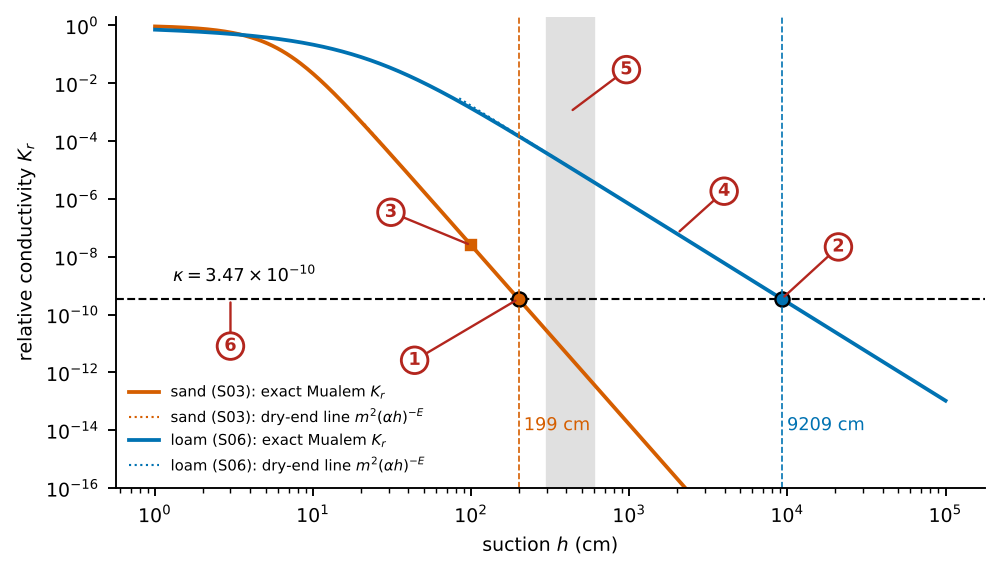
\includegraphics[width=0.92\textwidth]{../figures/paper4/ex_kr.png}\end{center}
\textbf{What the numbered labels point to, with the exact values.}
\begin{enumerate}[nosep,label=\protect\circled{\arabic*}]
\item Sand: the exact curve crosses the dashed line $K_r=\kappa$ at $h_c=199$\,cm (dot). This is \cref{eq:s-hc} with $\alpha=0.145$, $n=2.68$, $\ell=0.5$.
\item Loam: the crossing is at $h_c=9\,209$\,cm, just below $10^4$\,cm, with $\alpha=0.036$, $n=1.56$.
\item Sand at field capacity (100\,cm): $K_r=2.5\times10^{-8}$, a fraction of the saturated conductivity that is already tiny; the worked example of Part~2 of the guide.
\item Dotted lines: the dry-end straight line $m^2(\alpha h)^{-E}$. It lies on the exact curve wherever $\alpha h\gg1$, which is why the closed form of the reach is accurate.
\item Grey band (300--600\,cm): the usual triggers. They lie beyond the reach of sand and well inside the reach of loam.
\item The constant $\kappa$: the relative conductivity below which a crop can no longer dry the soil at the sensor within a season; one value for all ten soils.
\end{enumerate}
\textbf{How the exact points are obtained from the data.} The curves are the Mualem conductivity computed from $\alpha$ and $n$ of each soil (Table~A1 of the article, \nolinkurl{Manuscripts/results/p4_tableA1_reach.csv}). $\kappa$ is the fitted constant of \nolinkurl{p4_numbers.json} (key \texttt{kappa}), obtained from experiment E2 as shown in the next graph. The two crossings are computed with \cref{eq:s-hc}; the same numbers are in the workbook sheet \texttt{EQ\_P4\_reach}, cells of S03 and S06.

\subsection{Exact points: how the single constant $\kappa$ is found}
The loss counts, for every soil, how many decades the predicted reach lies outside the interval observed in the simulations (zero when inside), squared and summed. The constant is the value of $\kappa$ at the bottom of this curve.
\begin{center}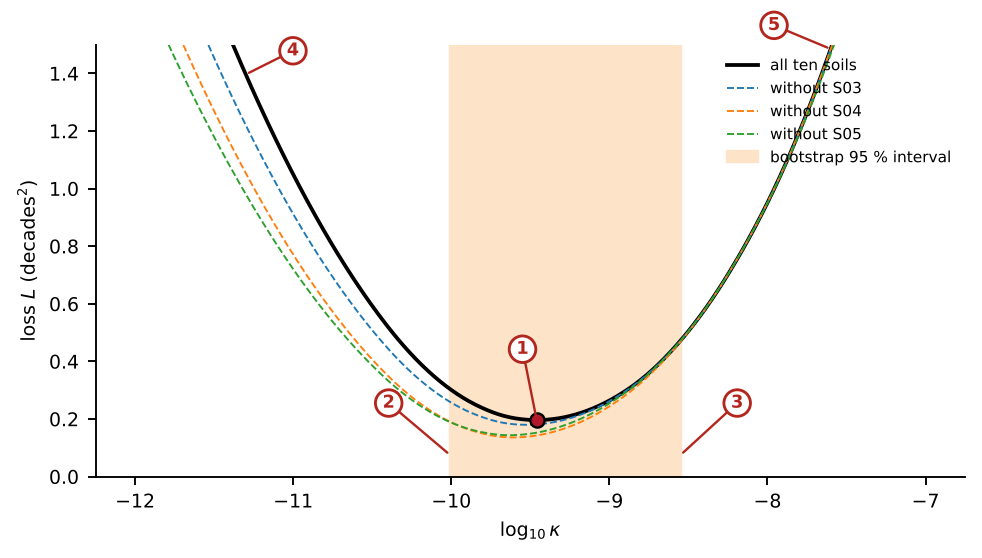
\includegraphics[width=0.92\textwidth]{../figures/paper4/ex_kappa.png}\end{center}
\textbf{What the numbered labels point to, with the exact values.}
\begin{enumerate}[nosep,label=\protect\circled{\arabic*}]
\item The minimum: $\log_{10}\kappa=-9.46$, $\kappa=3.47\times10^{-10}$, loss $L=0.196$\,decades$^2$. At this value 5 soils lie outside their interval: S01 by 0.11 decade, S02 by 0.27 decade, S03 by 0.12 decade, S04 by 0.23 decade, S05 by 0.21 decade; the other 5 lie inside.
\item Left edge of the bootstrap interval, $\kappa=9.8e-11$: resampling the ten soils with replacement 1\,000 times and refitting.
\item Right edge, $\kappa=2.8e-09$. The interval spans 1.5 decades, but the reach changes only by a factor 1.45 to 2.45 per decade of $\kappa$.
\item Too small a $\kappa$ puts every predicted reach too far into the dry range: the soils with a finite interval (sand, loamy sand, sandy loam) are missed and the loss rises.
\item Too large a $\kappa$ predicts reaches that are too short: soils whose triggers fire up to $10^4$\,cm are missed.
\end{enumerate}
\textbf{How the exact points are obtained from the data.} The observed intervals are the columns \texttt{reach\_observed\_low\_cm} and \texttt{reach\_observed\_high\_cm} of Table~A1, from experiment E2 (next graph). The predicted reach for each trial $\kappa$ is \cref{eq:s-hc}. The minimum was found with the Nelder--Mead method in \nolinkurl{p4_reach.py} (function \texttt{fitm}); the bootstrap and the curves without one soil are in \nolinkurl{p4_numbers.json} under \texttt{constants}. The flat bottom of the curve is why $\kappa$ is uncertain by a decade while the reaches are not: every reach depends on $\kappa$ only through the power $1/[2n+\ell(n-1)]$.

\subsection{The constant $\kappa$ of the reach: how it is determined}
\begin{problem}[title={What $\kappa$ is}]
$\kappa$ is the relative conductivity $K_r=K/K_s$ at which the crop can no longer dry the soil at the sensor within a season. It is the only constant of \cref{eq:s-hc}. It is \emph{not} measured directly: it is found from the simulated triggers, in five steps.
\end{problem}
\begin{derivation}[title={How $\kappa$ was determined, step by step}]
\textbf{Step 1: the experiment.} Experiment E2 (197 valid runs) sets the trigger to 20 values from 50 to 10\,000\,cm on each of the ten soils. Everything else is fixed: the sensor at 20\,cm, a dose of 2.4\,mm per event, surface application, the crop file \texttt{crops\_conv\_N100.dai} (the cereal rotation of the ensemble under conventional tillage with 100\,kg\,N\,ha$^{-1}$), and 20 years of Taastrup weather (1980--1999).

\textbf{Step 2: when does a trigger fire?} A trigger is counted as firing on a soil if it brings at least 5\,mm of irrigation a year (20-year mean).

\textbf{Step 3: the observed reach of each soil.} For each soil the reach lies between the driest trigger that still fires ($h_{\mathrm{lo}}$) and the next drier one, which does not ($h_{\mathrm{hi}}$); if even 10\,000\,cm fires, only $h_{\mathrm{lo}}$ is known. Sand: 100--150\,cm; loamy sand: 200--250\,cm; sandy loam: 800--1\,000\,cm; loam and sandy clay loam: 5\,000--10\,000\,cm; the five finer or coarse-loamy soils: above 10\,000\,cm.

\textbf{Step 4: one $\kappa$ for all soils.} For a trial $\kappa$, \cref{eq:s-hc} gives a reach for every soil. Its distance to the observed interval is measured in decades (zero if inside, the distance to the nearer end if outside), squared and added over the ten soils.

\textbf{Step 5: the best $\kappa$.} The sum is minimised over $\log_{10}\kappa$ with the Nelder--Mead method. The minimum is at $\kappa=3.47\times10^{-10}$.
\end{derivation}
\begin{keyresult}[title={How certain $\kappa$ is}]
\centering\footnotesize
\begin{tabular}{>{\raggedright\arraybackslash}p{4.3cm}>{\raggedright\arraybackslash}p{5.2cm}>{\raggedright\arraybackslash}p{4.0cm}}
\toprule
Test & Result & What it means\\\midrule
Bootstrap over soils (1\,000 resamples) & $\kappa$ between $1.0\times10^{-10}$ and $2.8\times10^{-9}$ (95\,\%) & $\kappa$ is known to about one decade\\
Leaving each soil out & $2.3\times10^{-10}$ to $7.3\times10^{-10}$ & no single soil decides $\kappa$\\
Firing threshold 1 or 2\,mm & $2.7\times10^{-10}$ & a stricter count changes $\kappa$ little\\
Firing threshold 5\,mm (used) & $3.5\times10^{-10}$ & \\
Firing threshold 10\,mm & $7.3\times10^{-10}$ & \\
Firing threshold 20\,mm & $1.3\times10^{-9}$ & \\
Firing threshold 40\,mm & $2.5\times10^{-9}$ & a looser count raises $\kappa$\\\bottomrule
\end{tabular}
\end{keyresult}
\begin{pins}[title={How much an error in $\kappa$ moves the reach}]
\pin{1}{Because $\hc\propto\kappa^{-1/E}$, a tenfold error in $\kappa$ changes the reach by the factor $10^{1/E}$: 1.45 in sand, 1.56 in loamy sand, 1.73 in sandy loam, 1.97 in loam and 2.45 in silty clay loam. The reach is least sensitive exactly in the coarse soils where it matters most (where it decides whether a 300\,cm trigger works).}
\pin{2}{Moving the firing threshold from 5 to 20\,mm a year raises $\kappa$ about fourfold and shortens the reaches by a factor of 1.2 (sand) to 1.4 (silty clay loam); sand and loamy sand remain blind to a 300\,cm trigger with any threshold tested.}
\end{pins}
\begin{keyresult}[title={What $\kappa$ depends on}]
\textbf{Not the soil.} One value fits ten soils from sand to silty clay loam within a factor of 2.3, and the soil enters only through $\alpha$, $n$ and $\ell$.

\textbf{The crop: yes, in principle.} $\kappa$ expresses when the roots can no longer extract water from the soil around the sensor. It depends on the root length density at the sensor depth, the potential transpiration of the crop and the lowest root water potential the crop can sustain. A crop with denser or deeper roots, or one that tolerates lower water potentials, can dry the soil further, which means a smaller $\kappa$ and a longer reach. All runs of E2 used one cereal rotation, so the size of this effect was not measured.

\textbf{The climate: yes.} A higher evaporative demand stresses the crop earlier; the weather was one series (Taastrup), so this was not measured either.

\textbf{The sensor depth and the dose: yes.} The sensor was at 20\,cm, where the roots are dense; a deeper sensor sees fewer roots and dries less (in E3 a deeper sensor did not make sand irrigate at 300\,cm). The dose was 2.4\,mm.

\textbf{In practice.} $\kappa$ is a constant of the crop--climate--sensor system, not of the soil. For another crop or climate it is determined in the same way, with a trigger experiment of the kind of E2 on two or three soils, which the Daisy workbench of SWAFL Desktop can run.
\end{keyresult}


\subsection{Exact points: the observed reach in experiment E2}
Experiment E2 runs the same crop rotation and weather with one suction trigger at a time. Each dot is one run: its trigger and the irrigation it brought per year.
\begin{center}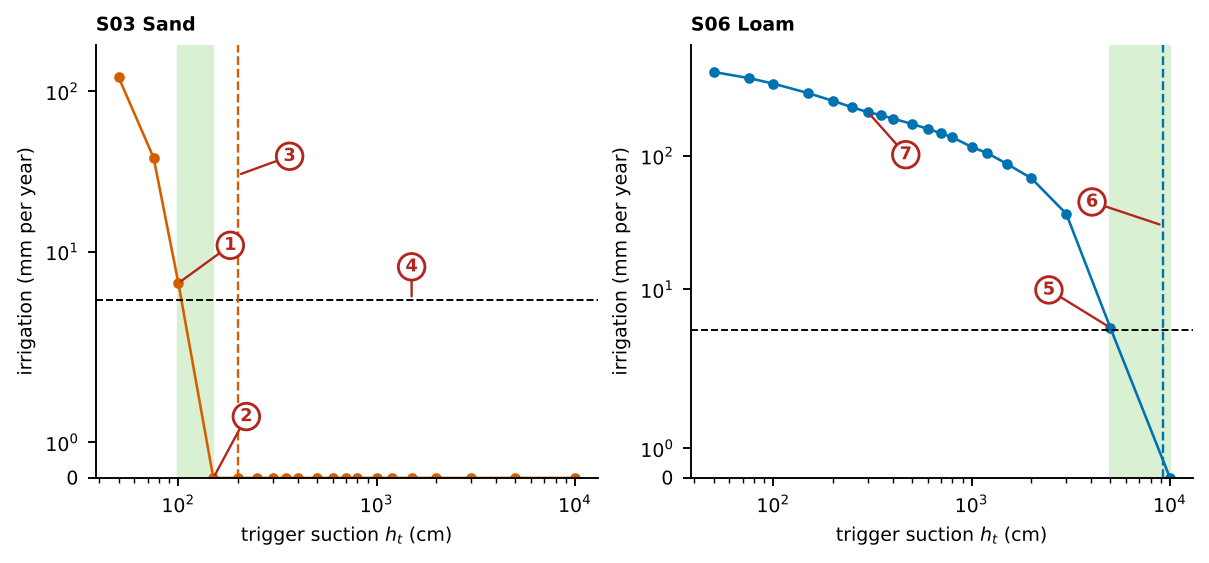
\includegraphics[width=0.92\textwidth]{../figures/paper4/ex_e2.png}\end{center}
\textbf{What the numbered labels point to, with the exact values.}
\begin{enumerate}[nosep,label=\protect\circled{\arabic*}]
\item Sand, the driest trigger that still fires: 100\,cm brings 6.36\,mm a year, above the 5\,mm line.
\item Sand, the next trigger, 150\,cm, brings 0.0\,mm: it never fires. The observed reach lies between the two (green band, 100--150\,cm).
\item The reach predicted by the closed form, 199\,cm (dashed): a third above the band, the largest miss among the soils with a finite interval.
\item The 5\,mm a year threshold that defines ``fires; with 1, 10, 20 or 40\,mm the fitted $\kappa$ becomes 2.7, 7.3, 13 or 25 $\times10^{-10}$.
\item Loam, the driest trigger that fires: 5000\,cm brings 5.16\,mm a year.
\item Predicted reach of loam, 9\,209\,cm: inside the observed band 5\,000--10\,000\,cm.
\item Loam at the usual 300\,cm trigger: 212\,mm a year of irrigation, the trigger works.
\end{enumerate}
\textbf{How the exact points are obtained from the data.} E2 is the experiment \texttt{E2\_TriggerPressure} of \nolinkurl{Data/Comprehensive_Summary/00_summary_all_simulations.csv.gz}: 10 soils $\times$ 20 triggers (20 to 10\,000\,cm), sensor at 20\,cm, dose 2.4\,mm, crop file \texttt{crops\_conv\_N100.dai}, weather Taastrup 1980--1999. For each soil the script \nolinkurl{p4_reach.py} takes the column \texttt{set\_trigger\_potential\_cm} (sign changed) and \texttt{irrigation\_mm}; the largest trigger with at least 5\,mm a year is the lower end of the interval, the next larger trigger the upper end. These points are in \nolinkurl{p4_fig3_trigger_runs.csv}.

\subsection{Reading Figure 1 of the article}
\begin{center}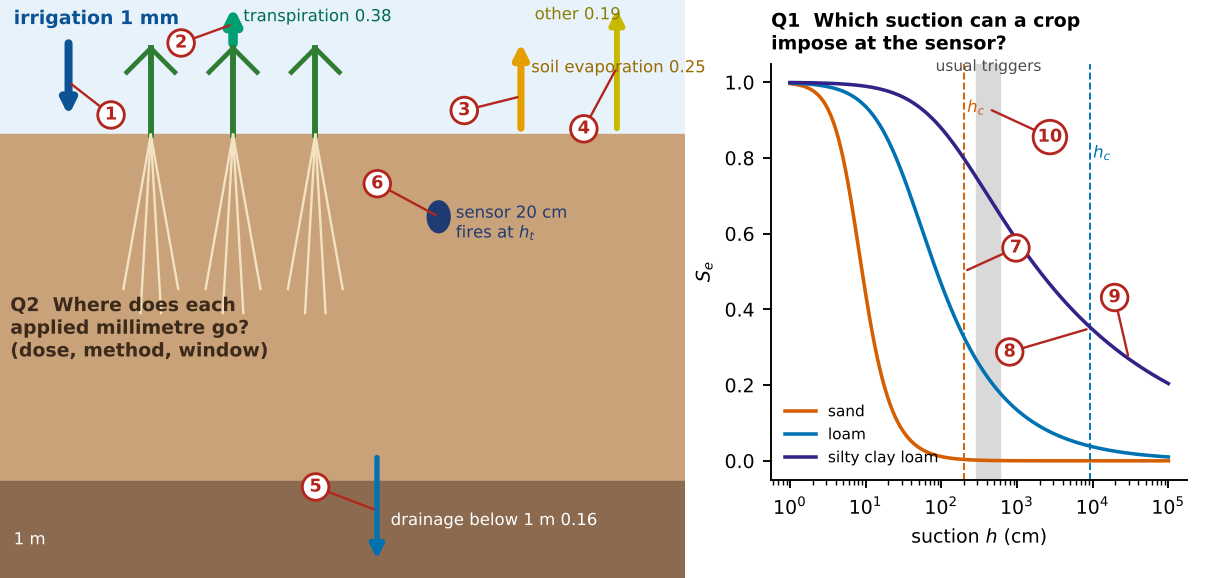
\includegraphics[width=\textwidth,height=0.42\textheight,keepaspectratio]{../figures/paper4/fig1_concept_annot.png}\end{center}

\textbf{What the numbered labels point to.}
\begin{enumerate}[nosep,label=\protect\circled{\arabic*}]
\item One millimetre of irrigation applied to the surface; the arrows that leave the column are its fates, with widths in proportion to their shares.
\item Transpiration (0.38 of each millimetre): the only fate that makes yield.
\item Soil evaporation (0.25): water evaporated from the wetted surface with the energy also available to the crop.
\item Other evaporation (0.19): intercepted water, ponds and litter.
\item Drainage below 1 m (0.16): water lost to the crop that also carries nitrate.
\item The sensor at 20 cm: irrigation starts when the suction it reads exceeds the trigger.
\item The reach of sand (199 cm, the dashed orange line): there its conductivity has collapsed; the usual triggers (grey band) lie beyond it and never fire.
\item The reach of loam (9 209 cm, the dashed blue line just below $10^4$ cm): its gentler curve lets a crop dry it far further, so the usual triggers lie well inside its reach and fire.
\item Silty clay loam: its reach (128 260 cm) lies beyond the right edge of the axis ($10^5$ cm), so no dashed line is drawn; every usual trigger fires.
\item Grey band: the triggers usually tabulated (300 to 600 cm).
\end{enumerate}

\textbf{What it shows.} The two questions. Q1 (right): a trigger $\htr$ fires only if the crop can dry the soil at the sensor to $\htr$; the reach $\hc$ (dashed) is 199\,cm in sand and $9\times10^{3}$\,cm in loam, so the usual triggers (grey) lie beyond the reach of sand. Q2 (left): the fate of an irrigation millimetre, averaged over the 744 irrigated runs of experiment E10 (arrow widths to scale).

\textbf{How to read the labels, symbols and colours.} Left: a soil column with three crops; the blue arrow is one millimetre of irrigation and the coloured arrows leaving the column are its fates, drawn with widths in proportion to their shares (green transpiration, orange soil evaporation, yellow other evaporation, blue drainage below 1\,m). The dark dot is the sensor at 20\,cm. Right: effective saturation $S_e$ against suction $h$ (log axis) for sand, loam and silty clay loam; the dashed vertical line of each colour is that soil's reach $\hc$; the grey band is the range of triggers usually tabulated (300 to 600\,cm).

\textbf{What affects it, and why it happens.} The sand curve falls to almost zero within a few tens of centimetres, so its conductivity collapses early and its reach (199\,cm) lies to the left of the usual triggers: such a trigger is never read. In the loam the reach lies far to the right, so the same triggers work. The arrow widths show that less than half of an applied millimetre is transpired because the same energy also evaporates water from the soil and from intercepted or ponded water.

\textbf{How it is made.} Schematic drawn by the script with numbers from the results. Script: \nolinkurl{Manuscripts/reproducibility/analysis/p4_concept.py}. Input: \nolinkurl{Data/Comprehensive_Summary/00_summary_all_simulations.csv.gz}.


\subsection{Reading Figure 2 of the article}
\begin{center}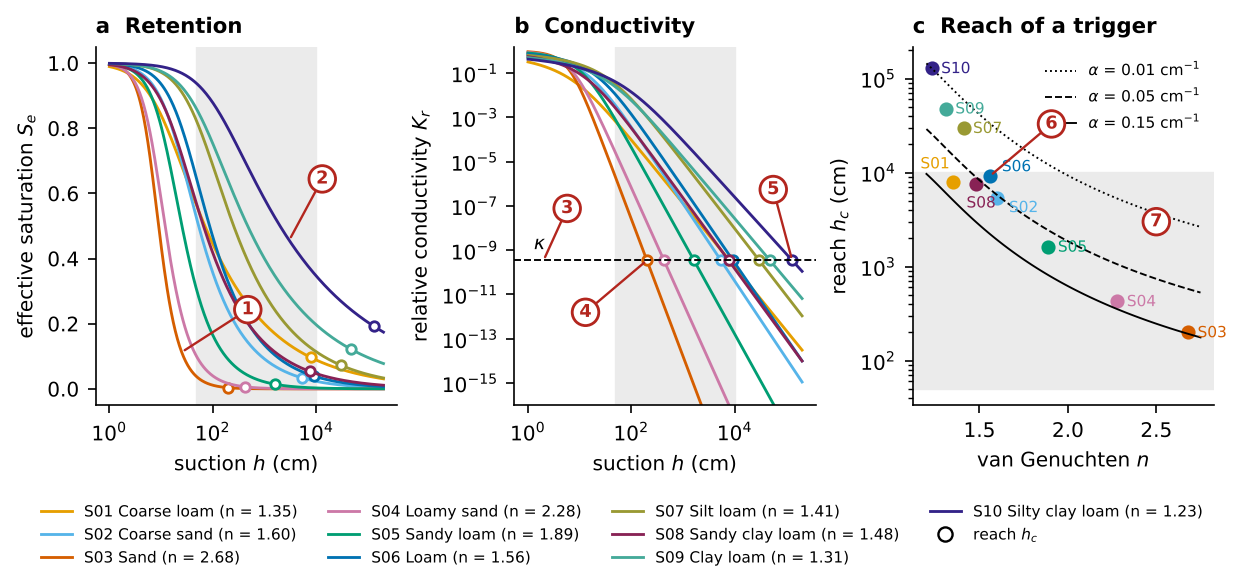
\includegraphics[width=\textwidth,height=0.42\textheight,keepaspectratio]{../figures/paper4/fig2_curves_reach_annot.png}\end{center}

\textbf{What the numbered labels point to.}
\begin{enumerate}[nosep,label=\protect\circled{\arabic*}]
\item Sand: its retention curve drops almost to zero within a few tens of centimetres of suction, because its pores are nearly all the same size (large n = 2.68).
\item Silty clay loam: the curve falls slowly over five decades of suction, because its pores span many sizes (small n = 1.23).
\item The dashed line is the constant $\kappa=3.47\times10^{-10}$: the relative conductivity at which a crop can no longer dry the soil at the sensor.
\item The reach of sand (199 cm) is where its conductivity curve crosses $\kappa$; the steep curve crosses early.
\item The reach of silty clay loam (128 260 cm): its gentle curve crosses $\kappa$ only far in the dry range.
\item Each point is the reach of one soil from Eq. (4); the reach falls as n grows. The three lines are Eq. (4) for three values of $\alpha$: a smaller $\alpha$ gives a longer reach.
\item Grey band: the range of triggers tested in the simulations (50 to 10 000 cm). Soils whose reach lies inside the band have a trigger beyond which irrigation stops.
\end{enumerate}

\textbf{What it shows.} (a) Retention and (b) relative conductivity of the ten soils (Eq.~(1) and Eq.~(2) of the article); circles mark the reach of Eq.~(4) of the article and the dashed line the fitted $\kappa=3.5\times10^{-10}$; grey: the range of triggers tested. (c) Reach against $n$ for the ten soils, with Eq.~(4) of the article for three values of $\alpha$.

\textbf{How to read the labels, symbols and colours.} (a) $S_e$ against $h$ for the ten soils (colours in the legend, with each soil's $n$). (b) Relative conductivity $K_r$ against $h$, both on log scales; the dashed line is $\kappa$. Open circles in (a) and (b) mark each soil's reach. Grey shading: the range of triggers tested in the simulations (50 to 10\,000\,cm). (c) Reach against $n$ (log scale) for the ten soils (labelled points) and Eq.~(4) of the article for three values of $\alpha$ (dotted, dashed and solid lines).

\textbf{What affects it, and why it happens.} The reach is where each conductivity curve in (b) crosses the dashed line $\kappa$. Curves of large $n$ (sands) fall steeply and cross early; curves of small $n$ (silty clay loam) fall gently and cross late. In (c) the reach therefore falls with $n$, and for equal $n$ a smaller $\alpha$ (soil that starts draining later) gives a longer reach, which is why the three lines are ordered.

\textbf{How it is made.} Figure drawn by the script from the input data. Script: \nolinkurl{Manuscripts/reproducibility/analysis/p4_reach.py}. Input: \nolinkurl{Data/Comprehensive_Summary/00_summary_all_simulations.csv.gz}.


\subsection{Reading Figure 3 of the article}
\begin{center}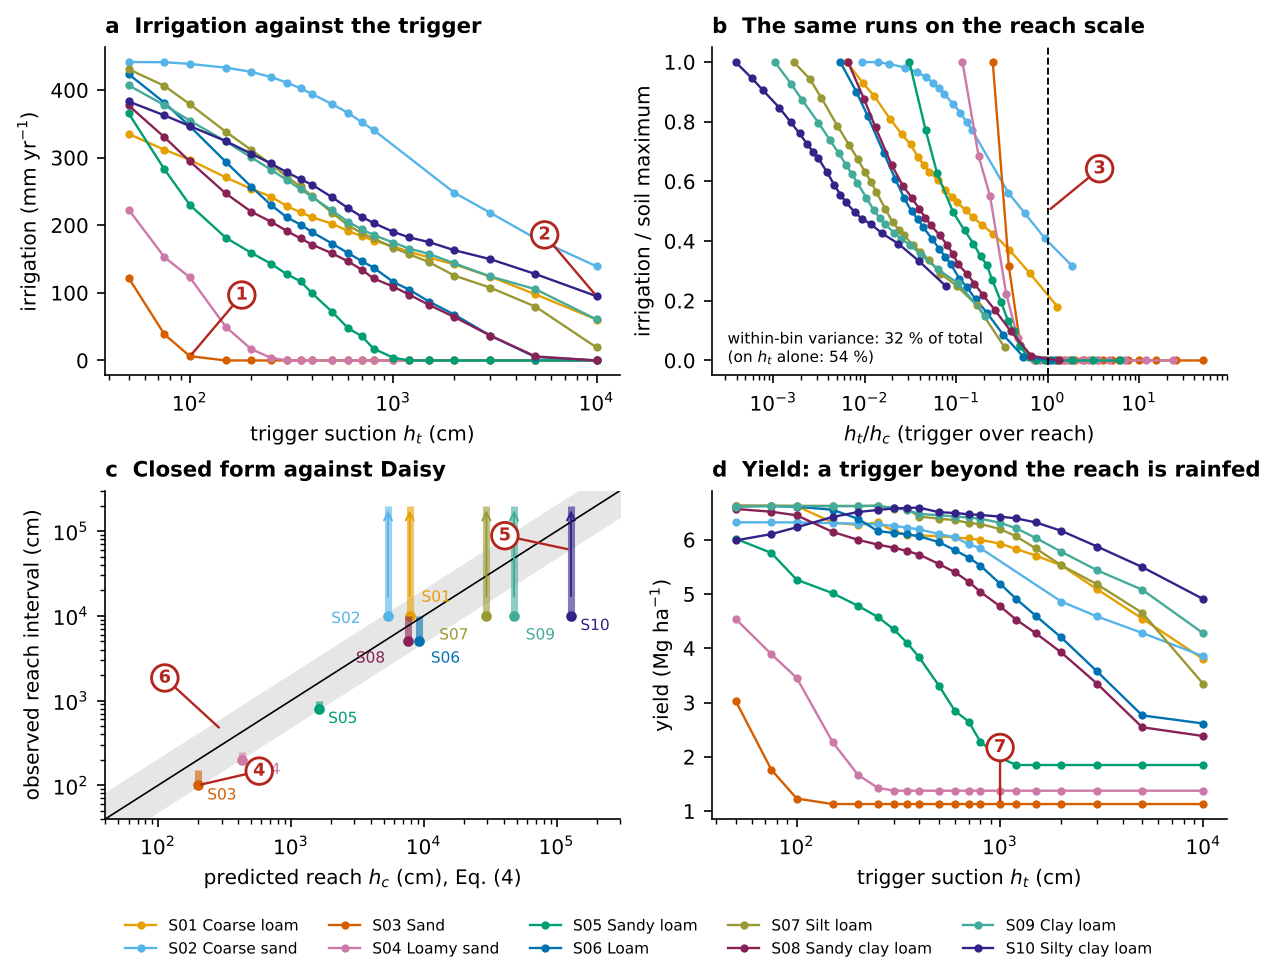
\includegraphics[width=\textwidth,height=0.42\textheight,keepaspectratio]{../figures/paper4/fig3_trigger_reach_annot.png}\end{center}

\textbf{What the numbered labels point to.}
\begin{enumerate}[nosep,label=\protect\circled{\arabic*}]
\item Sand: irrigation falls to zero at 100 to 150 cm. Every drier trigger, including the common 300 cm, is never reached.
\item Silty clay loam still irrigates at 10 000 cm, because its conductivity fades slowly and the crop can keep drying the soil.
\item The dashed line is the reach (trigger / reach = 1). On this scaled axis every soil stops irrigating between 0.5 and 1.
\item Sand: the bar is the observed interval (100 to 150 cm) and the dot its lower end; the prediction of Eq. (4) (199 cm) lies within a factor of two.
\item An arrow means that even the driest trigger tested (10 000 cm) still fired, so only a lower bound of the reach is known.
\item Grey band: within a factor of two of the 1:1 line (black). Points in the band are predicted well.
\item Sand beyond its reach: the yield stays at the rainfed value (1.13 Mg/ha) because the field is never irrigated.
\end{enumerate}

\textbf{What it shows.} The reach of a suction trigger in experiment E2 (197 runs). (a) Irrigation against the trigger. (b) The same runs against the reach-scaled trigger $\htr/\hc$, irrigation divided by its soil maximum: every soil stops at $\htr/\hc\approx0.5$ to 1. (c) Predicted reach (Eq.~(4) of the article) against the observed interval (bars; arrows: only a lower bound); grey band: within a factor of 2. (d) Yield against the trigger: beyond the reach the crop is rainfed.

\textbf{How to read the labels, symbols and colours.} (a) Annual irrigation (mm) against the trigger suction (log axis), one line per soil. (b) The same irrigation divided by each soil's maximum, against the trigger divided by the reach; the dashed line is $x=1$. (c) Predicted reach (Eq.~(4) of the article) against the observed interval: bars span the interval, arrows mean only a lower bound is known, the black line is 1:1 and the grey band a factor of two. (d) Yield against the trigger.

\textbf{What affects it, and why it happens.} Irrigation falls as the trigger becomes drier and stops at a cliff whose position follows the soil's conductivity (a). On the scaled axis every soil stops between 0.5 and 1 (b), because the reach captures where uptake stops. Points near the 1:1 line in (c) show the closed form places the cliffs within a factor of about two. In (d) yields stay at the rainfed value for triggers beyond the reach (sand, loamy sand), because the field is never irrigated.

\textbf{How it is made.} Figure drawn by the script from the input data. Script: \nolinkurl{Manuscripts/reproducibility/analysis/p4_reach.py}. Input: \nolinkurl{Data/Comprehensive_Summary/00_summary_all_simulations.csv.gz}.


\subsection{Derivation: The van~Genuchten--Mualem pair from a capillary bundle}\label{der:s4:1}
A soil is idealised as a bundle of capillaries whose radii are distributed so that the water-filled fraction at suction $h$ is the effective saturation $S_e$. The capillary (Young--Laplace) law relates the radius $r$ of the largest filled pore to the suction, $r=2\sigma\cos\gamma/(\rho_w g h)$, so $h\propto1/r$. \citet{Mualem1976} wrote the relative conductivity of such a medium as the product of a tortuosity--connectivity term $S_e^{\ell}$ and the square of a normalised integral of the pore radius over the filled pores:
\begin{equation}
K_r(S_e)=S_e^{\ell}\left[\frac{\int_0^{S_e}h(x)^{-1}\,\dd x}{\int_0^{1}h(x)^{-1}\,\dd x}\right]^{2}. \label{eq:s-mualem}
\end{equation}
\citet{vanGenuchten1980} chose the retention function $S_e=[1+(\alpha h)^n]^{-m}$, whose inverse is
\begin{equation}
h(x)=\frac{1}{\alpha}\bigl(x^{-1/m}-1\bigr)^{1/n}. \label{eq:s-inv}
\end{equation}
Substituting \cref{eq:s-inv} and $y=x^{1/m}$ ($x=y^{m}$, $\dd x=m\,y^{m-1}\dd y$):
\begin{equation}
\int_0^{S_e}\frac{\dd x}{h(x)}=\alpha m\int_0^{S_e^{1/m}}\bigl(y^{-1}-1\bigr)^{-1/n}y^{m-1}\,\dd y=\alpha m\int_0^{S_e^{1/m}}y^{\,m-1+1/n}(1-y)^{-1/n}\,\dd y .
\end{equation}
With the restriction $m=1-1/n$ the exponent of $y$ vanishes and $(1-y)^{-1/n}=(1-y)^{m-1}$, so the integral is elementary:
\begin{equation}
\int_0^{S_e}\frac{\dd x}{h(x)}=\alpha m\int_0^{S_e^{1/m}}(1-y)^{m-1}\dd y=\alpha\Bigl[1-\bigl(1-S_e^{1/m}\bigr)^{m}\Bigr].
\end{equation}
The denominator of \cref{eq:s-mualem} is the same expression at $S_e=1$, that is $\alpha$, and the closed form of the paper follows:
\begin{equation}
K_r(S_e)=S_e^{\ell}\Bigl[1-\bigl(1-S_e^{1/m}\bigr)^{m}\Bigr]^{2}. \label{eq:s-kr}
\end{equation}
This is why the restriction $m=1-1/n$ is not a convenience: it is the condition under which the Mualem integral has a closed form.


\subsection{Derivation: The dry-end asymptote of the conductivity}\label{der:s4:2}
For $\alpha h\gg1$, $(\alpha h)^n$ dominates the bracket of the retention function and
\begin{equation}
S_e=\bigl[1+(\alpha h)^n\bigr]^{-m}=(\alpha h)^{-mn}\bigl[1+(\alpha h)^{-n}\bigr]^{-m}=(\alpha h)^{-(n-1)}\Bigl[1-m(\alpha h)^{-n}+O\bigl((\alpha h)^{-2n}\bigr)\Bigr],
\end{equation}
since $mn=n-1$. Write $u=S_e^{1/m}$, which is small. The binomial expansion $(1-u)^{m}=1-mu-\tfrac{m(1-m)}{2}u^2+O(u^3)$ gives
\begin{equation}
1-(1-u)^{m}=mu\Bigl[1+\tfrac{1-m}{2}u+O(u^2)\Bigr].
\end{equation}
Inserting into \cref{eq:s-kr},
\begin{equation}
K_r=m^{2}\,S_e^{\ell+2/m}\Bigl[1+(1-m)S_e^{1/m}+\dots\Bigr].
\end{equation}
The exponent is $(\ell+2/m)(n-1)=\ell(n-1)+2n$, because $(n-1)/m=n$. Hence
\begin{equation}
K_r(h)=m^{2}(\alpha h)^{-[2n+\ell(n-1)]}\Bigl[1+\varepsilon(h)\Bigr],\qquad \varepsilon(h)=O\bigl((\alpha h)^{-n}\bigr)+O\bigl((\alpha h)^{-n}\bigr), \label{eq:s-asym}
\end{equation}
where both correction terms are of the order $(\alpha h)^{-n}$ (the first from the retention bracket, the second from $S_e^{1/m}=(\alpha h)^{-n}[1+\dots]$). For the soils of the paper the reach lies at $\alpha\hc$ between 29 and 1\,280, where $(\alpha\hc)^{-n}$ is below $10^{-3}$: the asymptote is exact to better than one per mille at the reach.


\subsection{Derivation: The reach of a trigger}\label{der:s4:3}
\paragraph{The physical condition.} During a drying cycle the crop takes water from the layer that holds the sensor at a rate $u$ limited by the conductance of the soil between the bulk soil and the root surface \citep{Gardner1960}. For a cylindrical root of radius $r_0$ in a soil cylinder of radius $r_1$, steady radial flow gives
\begin{equation}
u\simeq\frac{2\pi L_v}{\ln(r_1/r_0)}\int_{h_{\mathrm{root}}}^{h}K(h')\,\dd h' \;\approx\; \frac{2\pi L_v}{\ln(r_1/r_0)}\,K(h)\,\Delta h,
\end{equation}
with $L_v$ the root length density and $\Delta h$ the head drop to the root. Because $K$ falls by many decades while $\Delta h$ is bounded by the plant (the wilting point), $u$ collapses once $K(h)$ is small enough, and the soil at the sensor stops drying within the time of a season. The suction where this happens is the reach $\hc$.
\paragraph{One constant for all soils.} If the reach is reached at one value $\kappa$ of the relative conductivity, $K_r(\hc)=\kappa$, \cref{eq:s-asym} gives
\begin{equation}
\begin{gathered}m^{2}(\alpha\hc)^{-[2n+\ell(n-1)]}=\kappa\\ \Longrightarrow\quad \boxed{\;\hc=\frac{1}{\alpha}\Bigl(\frac{m^{2}}{\kappa}\Bigr)^{1/[2n+\ell(n-1)]}\;}\end{gathered} \label{eq:s-hc}
\end{equation}
\paragraph{Properties.} (i) $\alpha$ only rescales the reach: $\alpha\hc$ depends on $n$, $\ell$ and $\kappa$ alone. (ii) The logarithmic sensitivity to $n$ is
\begin{equation}
\frac{\partial\ln(\alpha\hc)}{\partial n}=\frac{2}{m\,n^{2}\,[2n+\ell(n-1)]}-\frac{(2+\ell)\ln(m^{2}/\kappa)}{[2n+\ell(n-1)]^{2}},
\end{equation}
whose second term dominates (with $\kappa=3.5\times10^{-10}$, $\ln(m^2/\kappa)\approx18$ to 21), so the reach shortens steeply as $n$ grows: from $\alpha\hc\approx1\,280$ at $n=1.23$ to $29$ at $n=2.68$. (iii) A larger $\ell$ shortens the reach because the conductivity collapses faster. (iv) For $n\to1$ the exponent tends to 2 and $m\to0$, so the reach tends to $\alpha^{-1}(m^{2}/\kappa)^{1/2}$, which vanishes slowly: very broad pore-size distributions are still reachable far into the dry range, as observed for the silty clay loam.


\subsection{Derivation: The alternative laws}\label{der:s4:4}
\paragraph{Fixed saturation.} If the reach were set by a water content, $S_e(\hc)=S_c$, inverting the retention function gives $\hc=\alpha^{-1}(S_c^{-1/m}-1)^{1/n}$. It ignores the conductivity and predicts the coarse soils worst (Table~2 of the paper).
\paragraph{Power law in $n-1$.} $\alpha\hc=A(n-1)^{-B}$ is an empirical two-parameter law; it fits slightly better but has no derivation.
\paragraph{Absolute conductivity.} $K(\hc)=K_s K_r(\hc)=q_c$ would give $\hc=\alpha^{-1}(m^{2}K_s/q_c)^{1/[2n+\ell(n-1)]}$. With literature $K_s$ the conductivity at the observed reaches spans more than three decades, so a single $q_c$ is rejected.


\subsection{Derivation: Fitting interval-censored reaches}\label{der:s4:5}
For each soil the data give an interval $[\,h_{\mathrm{lo}},h_{\mathrm{hi}})$: $h_{\mathrm{lo}}$ is the driest trigger that still brings at least 5\,mm of irrigation a year and $h_{\mathrm{hi}}$ the next drier trigger, or $+\infty$ when even the driest trigger fires. The loss of a prediction $\hat h$ is the squared distance in decades to the interval,
\begin{equation}
\mathcal L(\hat h)=\begin{cases}(\log_{10}h_{\mathrm{lo}}-\log_{10}\hat h)^2, & \hat h<h_{\mathrm{lo}},\\ 0, & h_{\mathrm{lo}}\le\hat h\le h_{\mathrm{hi}},\\ (\log_{10}\hat h-\log_{10}h_{\mathrm{hi}})^2, & \hat h>h_{\mathrm{hi}},\end{cases}
\end{equation}
summed over soils and minimised over $\log_{10}\kappa$ (Nelder--Mead). Leave-one-soil-out validation refits $\kappa$ without the soil and evaluates $\mathcal L$ on it; the reported error is $\sqrt{\mathcal L}$ in decades and the worst factor is $10^{\max\sqrt{\mathcal L}}$.


\subsection{Why it happens}
\paragraph{Why a trigger has a reach.} The crop can only dry the soil at the sensor as fast as the soil delivers water to the roots. That delivery scales with the conductivity, which falls by many orders of magnitude as the soil dries. In a soil with a narrow pore-size distribution (large $n$, sands) the conductivity collapses within a narrow band of suction just past the air entry, so the crop stops drying the soil there; whatever trigger is set beyond that band is never read. In a soil with a broad distribution (small $n$, silty clay loams) the conductivity fades slowly over many decades of suction and the crop can still dry the soil at very high suctions.

\paragraph{Why a deeper sensor does not help.} Below the sensor depth of the experiments the root density is smaller, so the soil dries even less, and in sands the deeper soil is also wetted by drainage from above. A deeper sensor therefore reads lower suctions, not higher ones.

\paragraph{Why scaling by the reach collapses the curves only in part.} The reach sets where irrigation ends, because it is fixed by the conductivity. How irrigation fades before the reach depends on how often the soil reaches a given suction in a season, which depends on the water held between field capacity and that suction, a retention property that differs from the conductivity property that sets the reach.

\section{The fate of an irrigation millimetre}
Where each applied millimetre goes, computed from irrigated runs and their rainfed twins, by soil, method and season.

\subsection{Contribution 4: the fate of an irrigation millimetre}\label{con:s4:4}
\begin{problem}
Of every millimetre of water pumped onto a field, how much does the crop transpire, and where does the rest go? The answer must hold for many soils, doses, seasons and methods, not for one case.
\end{problem}
\begin{derivation}
Write the 20-year balance of an irrigated run and of its rainfed twin (same soil and weather), subtract them, and divide by the irrigation $I$ (Section~\ref{der:s4:6}).
\end{derivation}
\begin{keyresult}
\begin{pencil}
{\small\noindent\textbf{How it is derived, line by line}
\[\begin{array}{@{}l@{}}\textbf{1. Balance of the irrigated run:}\\[1pt]
\qquad P+I=T+E_s+E_o+D+\Delta S+Q\\[1pt]
\textbf{2. Balance of the rainfed twin:}\\[1pt]
\qquad P=T_0+E_{s,0}+E_{o,0}+D_0+\Delta S_0+Q_0\\[1pt]
\textbf{3. Subtract 2 from 1 (}P\textbf{ cancels):}\\[1pt]
\qquad I=(T-T_0)+(E_s-E_{s,0})+(E_o-E_{o,0})\\ \qquad\quad+(D-D_0)+(\Delta S+Q-\Delta S_0-Q_0)\\[1pt]
\textbf{4. Divide by } I\textbf{:}\\[1pt]
\qquad 1=\eta_T+\eta_{E_s}+\eta_{E_o}+\eta_D+\eta_S
\end{array}\]}
\noindent\textbf{The result, with its parts marked}
\[
1=\underbrace{\eta_T}_{\circled{1}\ 0.38}+\underbrace{\eta_{E_s}}_{\circled{2}\ 0.25}+\underbrace{\eta_{E_o}}_{\circled{3}\ 0.19}+\underbrace{\eta_D}_{\circled{4}\ 0.16}+\underbrace{\eta_S}_{\circled{5}\ 0.03},\qquad \eta_X=\frac{\sum(X-X_0)}{\sum I}
\]
\end{pencil}
\centering\small
\begin{tabular}{lrrrr}
\toprule
Soil & transpired & soil evap. & other evap. & drained\\\midrule
Sandy loam & 0.64 & 0.11 & 0.14 & 0.07\\
Loam & 0.41 & 0.22 & 0.17 & 0.15\\
Coarse loam & 0.38 & 0.32 & 0.19 & 0.08\\
Coarse sand & 0.23 & 0.19 & 0.26 & \circled{6} 0.32\\\bottomrule
\end{tabular}
\end{keyresult}
\begin{pins}
\pin{1}{Only 38\,\% of irrigation becomes transpiration, the only flux that makes yield. Transpiration is capped by the energy reaching the canopy and by its cover.}
\pin{2}{A quarter evaporates from the wetted soil surface: water applied to bare or partly covered soil uses the same energy as transpiration.}
\pin{3}{Another fifth evaporates from ponded water, litter and intercepted water, the term usually left out of irrigation accounts.}
\pin{4}{Sixteen per cent drains below 1\,m and is lost to the crop (and carries nitrate).}
\pin{5}{The small remainder changes storage or runs off; it closes the balance and is a check of the calculation.}
\pin{6}{In coarse sand drainage is the largest single loss: the soil passes extra water on before the crop can use it.}
\end{pins}


\subsection{Contribution 6: overhead irrigation adds no transpiration}\label{con:s4:6}
\begin{derivation}
The identity of Contribution~4 was applied to the method experiments: E4 (surface, overhead and subsurface on every soil) and E15 (the three methods on coarse loam over all rates, doses and rooting depths), each run against its rainfed twin.
\end{derivation}
\begin{keyresult}
\begin{pencil}
{\small\noindent\textbf{How it is derived, line by line}
\[\begin{array}{@{}l@{}}\textbf{1. Identity of Contribution 4 for overhead runs:}\\[1pt]
\qquad \eta_T=\textstyle\sum(T-T_0)/\sum I\\[1pt]
\textbf{2. Data of E4 (all soils):}\\[1pt]
\qquad \textstyle\sum(T-T_0)<0\\[1pt]
\textbf{3. Hence:}\\[1pt]
\qquad \eta_T^{\text{overhead}}=-0.08
\end{array}\]}
\noindent\textbf{The result, with its parts marked}
\[\underbrace{\eta_T^{\text{overhead}}}_{\circled{1}}=-0.08\ \text{(all soils)}\]
\[\underbrace{\eta_{E_o}^{\text{overhead}}}_{\circled{2}}=0.79\]
\end{pencil}
\end{keyresult}
\begin{pins}
\pin{1}{A negative marginal transpiration: the crop transpires slightly \emph{less} with overhead irrigation than without.}
\pin{2}{Most of the water is intercepted by the canopy and evaporates with the energy that would have driven transpiration; interception replaces transpiration instead of adding to it. Subsurface application avoids this (0.51 transpired) but drains more (0.23).}
\end{pins}


\subsection{Worked numbers, part 7: where an irrigation millimetre goes}
Compare an irrigated run with the same soil and weather without irrigation (the rainfed baseline). The differences in each water flux, divided by the irrigation, tell what each millimetre became.
\emph{Example: one run on coarse loam} (dose 10\,mm, April to October). Irrigation $I=222.5$\,mm a year. Transpiration rose from 147.6 to 223.0\,mm, $+75.4$\,mm, so $\eta_T=75.4/222.5=0.34$. Drainage rose from 6.1 to 39.5\,mm, so $\eta_D=33.4/222.5=0.15$. Soil evaporation rose from 146.4 to 228.8\,mm, so $\eta_{E_s}=0.37$. Other evaporation (ET minus transpiration minus soil evaporation) rose from 172.8 to 193.3\,mm, so $\eta_{E_o}=0.09$. The four add to 0.95; the remaining 0.05 went to storage and runoff.
\emph{Pooling the 100 irrigated runs of that soil.} Add all transpiration (21\,328\,mm), subtract 100 times the rainfed value ($100\times147.6=14\,762$), and divide by all irrigation (17\,277\,mm): $\eta_T=6\,567/17\,277=0.38$. The sheet \texttt{EQ\_P4\_fate} does exactly this with \texttt{SUMIFS} for every soil.


\subsection{Exact points: the fate of the irrigation of one run}
The worked example of the guide (coarse loam, dose 10\,mm, April to October) drawn as one bar. Each segment is the difference between a flux of the irrigated run and the same flux of the rainfed run of the same soil and weather.
\begin{center}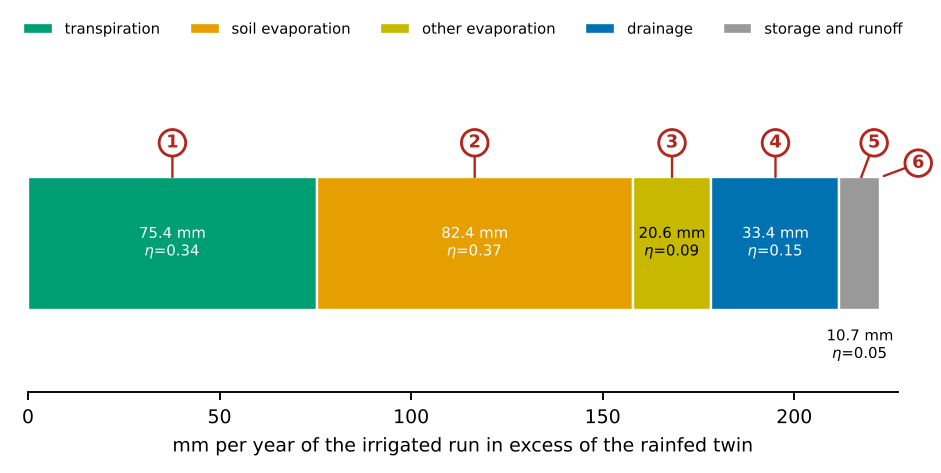
\includegraphics[width=0.92\textwidth]{../figures/paper4/ex_fate.png}\end{center}
\textbf{What the numbered labels point to, with the exact values.}
\begin{enumerate}[nosep,label=\protect\circled{\arabic*}]
\item Transpiration: 223.0 $-$ 147.6 = 75.4\,mm; $\eta_T=75.4/222.5=0.34$.
\item Soil evaporation: 82.4\,mm more than the rainfed twin; $\eta_{E_s}=0.37$, the largest share in this run because the surface is wetted every few days.
\item Other evaporation (interception, ponds, litter): 20.6\,mm; $\eta_{E_o}=0.09$.
\item Drainage below 1\,m: 39.5 $-$ 6.1 = 33.4\,mm; $\eta_D=0.15$.
\item The rest, 10.7\,mm, is the change of storage and runoff, obtained by difference so that the shares add to one.
\item The whole bar is the irrigation of the run, $I=222.5$\,mm a year: one bar is one irrigated millimetre scaled up.
\end{enumerate}
\textbf{How the exact points are obtained from the data.} The irrigated run is in experiment E10 and its rainfed twin in E0 (baseline of the same soil) of \nolinkurl{00_summary_all_simulations.csv.gz}; the columns used are \texttt{irrigation\_mm}, \texttt{transpiration\_mm}, \texttt{soil\_evap\_mm}, \texttt{ET\_mm} (other evaporation $=$ ET $-$ transpiration $-$ soil evaporation) and \texttt{drainage\_1m\_mm}; storage and runoff are $I-\Delta ET-\Delta D$. The article pools all irrigated runs of E10 of a soil (irrigation above 20\,mm a year) before dividing; the workbook sheet \texttt{EQ\_P4\_fate} repeats the pooled calculation with SUMIFS formulas.

\subsection{Reading Figure 4 of the article}
\begin{center}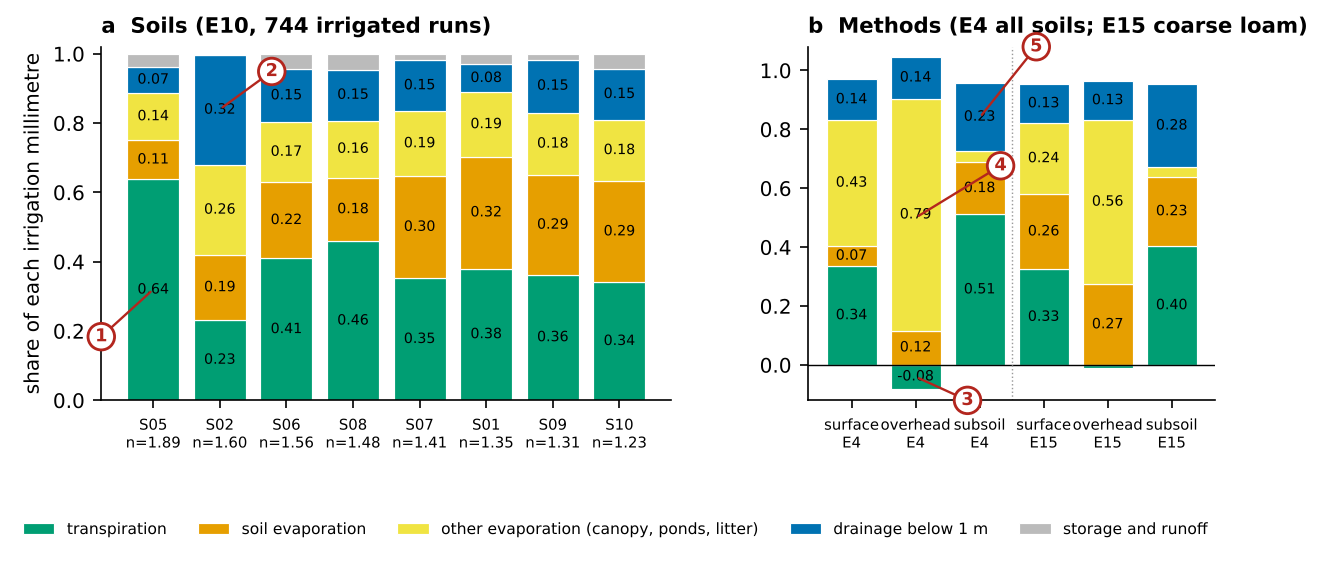
\includegraphics[width=\textwidth,height=0.42\textheight,keepaspectratio]{../figures/paper4/fig4_marginal_fate_annot.png}\end{center}

\textbf{What the numbered labels point to.}
\begin{enumerate}[nosep,label=\protect\circled{\arabic*}]
\item Sandy loam transpires the largest share of each irrigation millimetre (0.64): it holds the water near the roots and loses little to the surface.
\item Coarse sand: drainage below 1 m is the largest single loss (0.32), because the soil passes extra water on before the crop can use it.
\item Overhead irrigation: the transpired share is negative (-0.08). Water intercepted by the canopy evaporates with the energy that would have driven transpiration.
\item Most of the overhead water (0.79) leaves as other evaporation: canopy interception, ponds and litter.
\item Subsurface application transpires most (0.51) but also drains most (0.23), because it wets the profile from within.
\end{enumerate}

\textbf{What it shows.} The fate of an irrigation millimetre, Eq.~(5) of the article. (a) By soil (E10, 744 irrigated runs; sand and loamy sand are never irrigated at the 300\,cm trigger of E10), ordered by $n$. (b) By method, on all soils (E4) and on coarse loam over all rates, doses and rooting depths (E15).

\textbf{How to read the labels, symbols and colours.} Stacked bars of the shares of each irrigation millimetre: green transpiration, orange soil evaporation, yellow other evaporation (canopy, ponds, litter), blue drainage below 1\,m, grey storage and runoff; numbers inside the bars are the shares. (a) By soil, ordered by $n$ (label under each bar). (b) By method, on all soils (E4) and on coarse loam (E15); bars below zero are negative shares.

\textbf{What affects it, and why it happens.} Transpiration is limited by the energy reaching the canopy and by cover, so it takes less than half of the water. Coarse sand passes water on quickly, so drainage is its largest loss. Overhead irrigation wets the canopy; the intercepted water evaporates with the energy that would have driven transpiration, so the transpiration share is negative. Subsurface application avoids interception but wets the profile from within and drains more.

\textbf{How it is made.} Figure drawn by the script from the input data. Script: \nolinkurl{Manuscripts/reproducibility/analysis/p4_reach.py}. Input: \nolinkurl{Data/Comprehensive_Summary/00_summary_all_simulations.csv.gz}.


\subsection{Derivation: The marginal fate of irrigation}\label{der:s4:6}
For a run with irrigation $I$ and its rainfed twin (same soil, weather and crop), the 20-year water balances are
\begin{equation}
P+I=T+E_s+E_o+D+\Delta S+Q,\qquad P=T_0+E_{s,0}+E_{o,0}+D_0+\Delta S_0+Q_0 .
\end{equation}
Subtracting and dividing by $I$ gives the identity of the paper,
\begin{equation}
1=\underbrace{\frac{T-T_0}{I}}_{\eta_T}+\underbrace{\frac{E_s-E_{s,0}}{I}}_{\eta_{E_s}}+\underbrace{\frac{E_o-E_{o,0}}{I}}_{\eta_{E_o}}+\underbrace{\frac{D-D_0}{I}}_{\eta_D}+\underbrace{\frac{\Delta S-\Delta S_0+Q-Q_0}{I}}_{\eta_S}.
\end{equation}
The shares are marginal, not average: a share can be negative (overhead irrigation lowers transpiration) or exceed the average loss fraction. Pooling a group of runs uses the ratio of sums, $\eta_X=\sum(X-X_0)/\sum I$, which weights each run by its irrigation and is therefore the share of the group's total irrigation.


\subsection{Why it happens}
\paragraph{Why less than half of an irrigation millimetre is transpired.} Transpiration is limited by the energy available to the canopy and by the canopy cover. Water applied to a wet surface or to a canopy that does not cover the ground evaporates from the soil, from the ponded surface and from intercepted water, using the same energy; water applied beyond the storage of the root zone drains.

\paragraph{Why overhead irrigation adds no transpiration.} Water intercepted by the canopy evaporates with the energy that would otherwise drive transpiration, so the canopy transpires less while it is wet. The intercepted evaporation replaces transpiration rather than adding to it, and the marginal transpiration is nil or slightly negative.

\paragraph{Why early-season irrigation is more productive.} Early in the season the canopy is growing and its demand rises, so applied water is transpired; late in the season the cereal ripens and is harvested, and the same water is evaporated from bare soil or drains.


\section{The dose law}
How the share of a dose that drains grows with the size of the dose, and why the dose scale is nearly the same in every soil.

\subsection{Contribution 5: the dose law}\label{con:s4:5}
\begin{problem}
Small and frequent doses are recommended to reduce deep percolation. How small is small, and does the answer depend on the soil?
\end{problem}
\begin{derivation}
For each soil the drained share was computed at ten doses (1 to 30\,mm). A form was sought that is zero for a vanishing dose and levels off for a large one; the simplest is the saturating exponential, fitted per soil ($R^2$ 0.92 to 0.96 on seven soils).
\end{derivation}
\begin{keyresult}
\begin{pencil}
{\small\noindent\textbf{How it is derived, line by line}
\[\begin{array}{@{}l@{}}\textbf{1. A vanishing dose cannot drain:}\\[1pt]
\qquad \eta_D(0)=0\\[1pt]
\textbf{2. A large dose drains a soil-specific share:}\\[1pt]
\qquad \eta_D(\infty)=\eta_\infty\\[1pt]
\textbf{3. The extra share drained per extra mm falls in proportion to what is left:}\\[1pt]
\qquad \frac{\dd\eta_D}{\dd d}=\frac{\eta_\infty-\eta_D}{d_D}\\[1pt]
\textbf{4. Integrate with 1:}\\[1pt]
\qquad \eta_D(d)=\eta_\infty\bigl(1-e^{-d/d_D}\bigr)
\end{array}\]}
\noindent\textbf{The result, with its parts marked}
\[\eta_D(d)=\underbrace{\eta_\infty}_{\circled{1}}\Bigl(1-e^{-d/\underbrace{d_D}_{\circled{2}}}\Bigr)\]
\[\underbrace{\eta_D\approx\eta_\infty\,d/d_D\ \ (d\ll d_D)}_{\circled{3}}\]
\[\underbrace{d_D=4.1\pm0.6\text{ mm},\ \rho(d_D,n)=0.07}_{\circled{4}}\]
\end{pencil}
\end{keyresult}
\begin{pins}
\pin{1}{The plateau: the share of a large dose that drains. It differs between soils (0.10 to 0.20, and 0.45 in coarse sand) because it is the outcome of a race between drainage and uptake, which the soil's conductivity decides.}
\pin{2}{The dose scale: the dose at which 63\,\% of the plateau is reached. It is about 4\,mm in every soil.}
\pin{3}{For small doses the drained share grows in proportion to the dose: a dose much smaller than $d_D$ hardly drains, but in exchange most of it evaporates (60 to 72\,\% at 1\,mm).}
\pin{4}{$d_D$ is not related to $n$ or to any soil property: it is set by the atmosphere and the crop. Four millimetres is about one day of crop water use, so a dose below one day's use is consumed before it can move below the roots.}
\end{pins}


\subsection{Worked numbers, part 8: the dose law}
A small dose is used by the crop and the surface on the same day and cannot reach the deep soil; a large dose can. The share that drains therefore starts near zero and grows towards a ceiling $\eta_\infty$:
\[\eta_D(d)=\eta_\infty\bigl(1-e^{-d/d_D}\bigr).\]
\emph{Example (loam, $\eta_\infty=0.197$, $d_D=3.9$\,mm).} For a 1\,mm dose: $1/3.9=0.26$, $e^{-0.26}=0.77$, $1-0.77=0.23$, times 0.197 gives 0.045. For 10\,mm: $e^{-2.6}=0.074$, so $0.197\times0.926=0.18$. For 30\,mm: almost the ceiling, 0.197. The dose scale $d_D$ was about 4\,mm on every soil, close to one day of crop water use; the ceiling differs between soils (0.10 to 0.45).


\subsection{Exact points: the dose law of loam}
The worked example of Part~8 of the guide on its curve: the share of each irrigation millimetre that drains, against the dose applied at each event.
\begin{center}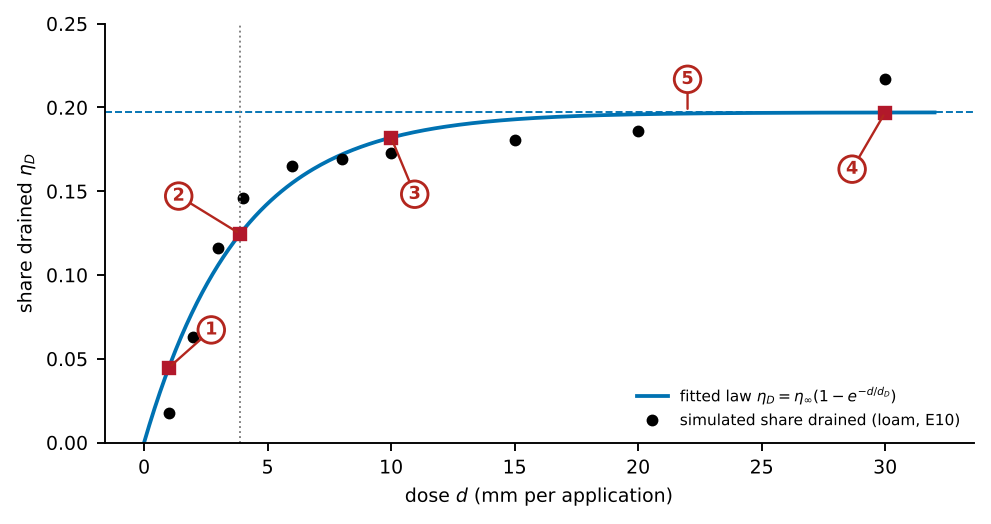
\includegraphics[width=0.92\textwidth]{../figures/paper4/ex_dose.png}\end{center}
\textbf{What the numbered labels point to, with the exact values.}
\begin{enumerate}[nosep,label=\protect\circled{\arabic*}]
\item $d=1$\,mm: $1-e^{-1/3.9}=0.23$; $\eta_D=0.045$. A small dose is used the same day and almost nothing drains.
\item $d=d_D=3.9$\,mm: by definition $\eta_D=\eta_\infty(1-e^{-1})=0.63\,\eta_\infty=0.125$.
\item $d=10$\,mm: $\eta_D=0.182$, already 92\,\% of the plateau.
\item $d=30$\,mm: $\eta_D=0.197$, practically the plateau.
\item The plateau $\eta_\infty=0.197$ of loam: the share of a large dose that drains, set by the race between drainage and uptake.
\end{enumerate}
\textbf{How the exact points are obtained from the data.} The black dots come from experiment E10 (\texttt{E10\_Amount\_Timing\_Soil}): the irrigated runs of loam are grouped by the dose per event (column \texttt{set\_dose\_mm\_per\_event}, 1 to 30\,mm, all irrigation windows pooled), and for each dose the summed extra drainage over the rainfed twin (E0) is divided by the summed irrigation. They are stored in \nolinkurl{p4_fig5_dose.csv}. The curve is the least-squares fit of the two parameters $\eta_\infty$ and $d_D$ (\texttt{scipy.optimize.curve\_fit} in \nolinkurl{p4_reach.py}); the fitted values and their standard errors are in \nolinkurl{p4_numbers.json} under \texttt{constants.dose\_fit}. The workbook sheet \texttt{EQ\_P4\_dose} evaluates the law at any dose.

\subsection{Reading Figure 5 of the article}
\begin{center}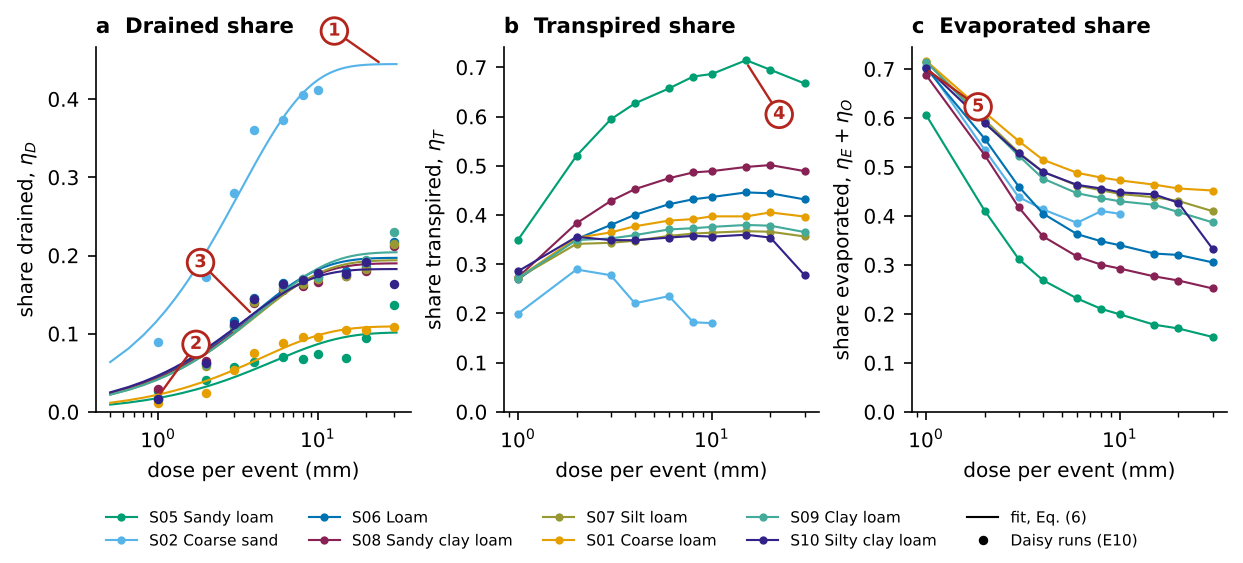
\includegraphics[width=\textwidth,height=0.42\textheight,keepaspectratio]{../figures/paper4/fig5_dose_annot.png}\end{center}

\textbf{What the numbered labels point to.}
\begin{enumerate}[nosep,label=\protect\circled{\arabic*}]
\item Plateau of coarse sand (0.45): the share of a large dose that drains. It is set by the soil, which passes water on fast.
\item Doses of 1 to 2 mm hardly drain (0.01 to 0.09): they are used near the surface on the day they are applied.
\item The dose scale $d_D$ (about 4 mm in every soil): at d = $d_D$ the drained share reaches 63 \% of its plateau. It is about one day of crop water use.
\item The transpired share rises with the dose and peaks at 15 to 20 mm, because less of a larger dose is lost from the wet surface.
\item At 1 mm, 60 to 72 \% of the dose evaporates: small doses trade drainage for evaporation.
\end{enumerate}

\textbf{What it shows.} The dose (E10, all ten windows pooled). (a) Drained share with Eq.~(6) of the article per soil. (b) Transpired share. (c) Evaporated share (soil and other evaporation).

\textbf{How to read the labels, symbols and colours.} Horizontal axes: dose per event (mm, log scale). (a) Drained share $\eta_D$: points are the Daisy runs (E10, pooled over windows), lines the fit of Eq.~(6) of the article. (b) Transpired share. (c) Evaporated share (soil plus other evaporation). Colours: soils, named in the legend.

\textbf{What affects it, and why it happens.} A dose smaller than one day of crop water use is consumed near the surface before it can drain, so $\eta_D$ is near zero at 1 to 2\,mm and the evaporated share is large. As the dose grows, more water reaches below the roots and the drained share rises to a plateau set by how fast the soil drains (highest in coarse sand). The transpired share rises with the dose because less of the water is lost from the surface.

\textbf{How it is made.} Figure drawn by the script from the input data. Script: \nolinkurl{Manuscripts/reproducibility/analysis/p4_reach.py}. Input: \nolinkurl{Data/Comprehensive_Summary/00_summary_all_simulations.csv.gz}.


\subsection{Derivation: The dose law}\label{der:s4:7}
Let a dose $d$ be applied when the root zone has a deficit. Part of the dose is used by the crop and the surface before it can move below the roots; the rest can drain. If the water that can be used before redistribution grows with the dose and saturates, and the drained share of the remainder is a soil property $\eta_\infty$, the simplest form with the right limits is
\begin{equation}
\eta_D(d)=\eta_\infty\bigl(1-e^{-d/d_D}\bigr),\qquad \eta_D\to\eta_\infty\frac{d}{d_D}\ (d\ll d_D),\qquad \eta_D\to\eta_\infty\ (d\gg d_D). \label{eq:s-dose}
\end{equation}
The small-dose limit is linear because a vanishing dose cannot drain; the large-dose limit is the share of any extra water that the soil passes on. The dose scale $d_D$ is the dose at which $1-e^{-1}=63\,\%$ of the plateau is reached. The form is phenomenological: it was chosen for its limits and tested against the data (coefficient of determination 0.92 to 0.96 on seven soils), not derived from the Richards equation.


\subsection{Why it happens}
\paragraph{Why the dose scale does not depend on the soil.} The water that a dose can lose to drainage is the part that the crop and the surface do not use before it redistributes below the roots. The crop uses about one day of evapotranspiration in that time whatever the soil, so the dose scale is set by the atmosphere and the crop and not by the soil.

\paragraph{Why the plateau depends on the soil.} Once a dose is large, the share that drains is the share of the excess that the soil passes on before the crop uses it, a race between drainage and uptake. Coarse sand passes water fast (high conductivity at field capacity), fine soils hold it, so the plateau is highest in coarse sand.

\section{When the lag of a sensor matters}
The non-equilibrium criterion for a suction trigger.

\subsection{Contribution 7: when a sensor's lag matters}\label{con:s4:7}
\begin{derivation}
The relaxation law of \citet{RossSmettem2000} was solved for a steady drying rate $r$: the water content lags by $r\tau$; dividing by the water capacity $C(h)$ turns this into a suction error; comparing the lag with the interval between irrigations gives the dimensionless number (Section~\ref{der:s4:8}).
\end{derivation}
\begin{keyresult}
\begin{pencil}
{\small\noindent\textbf{How it is derived, line by line}
\[\begin{array}{@{}l@{}}\textbf{1. Relaxation toward equilibrium:}\\[1pt]
\qquad \partial_t\theta=(\theta_{\mathrm{eq}}-\theta)/\tau\\[1pt]
\textbf{2. Steady drying } \partial_t\theta_{\mathrm{eq}}=-r\textbf{:}\\[1pt]
\qquad \theta=\theta_{\mathrm{eq}}+r\tau\\[1pt]
\textbf{3. Convert the water-content lag to suction:}\\[1pt]
\qquad \delta h=r\tau/C(h)\\[1pt]
\textbf{4. Compare the lag with the interval:}\\[1pt]
\qquad \Pi_\tau=\tau/t_i
\end{array}\]}
\noindent\textbf{The result, with its parts marked}
\[\underbrace{\Pi_\tau}_{\circled{1}}=\frac{\underbrace{\tau}_{\circled{2}}}{\underbrace{t_i}_{\circled{3}}},\qquad \delta h\simeq\frac{r\tau}{\underbrace{C(h)}_{\circled{4}}}\]
\end{pencil}
\end{keyresult}
\begin{pins}
\pin{1}{A dimensionless number: if it is much smaller than one, the equilibrium reach of Contribution~1 holds.}
\pin{2}{The relaxation time of the water content towards the retention curve (minutes to hours).}
\pin{3}{The interval between irrigations. Daily scheduling gives $\Pi_\tau\approx0.02$; pulses every half hour give $\Pi_\tau\approx2$.}
\pin{4}{The water capacity $C=-\dd\theta/\dd h$. It is smallest on the steep dry limb of a sand, so the same lag gives the largest error exactly where the reach is shortest. This criterion is proposed, not tested: Daisy solves equilibrium flow.}
\end{pins}

\subsection{Worked numbers, part 9: when the sensor's lag matters}
In fast wetting and drying the water content can lag behind the value of the retention curve by a time $\tau$. If the schedule irrigates every $t_i$ days, the lag matters only when $\Pi_\tau=\tau/t_i$ is not small. \emph{Example:} $\tau=1$\,h and irrigation every 2 days gives $\Pi_\tau=1/48=0.02$, negligible; pulses every 30\,min give $\Pi_\tau=2$, important.


\subsection{Derivation: Dynamic non-equilibrium and the lag of a sensor}\label{der:s4:8}
In the effective approach of \citet{RossSmettem2000} and \citet{Diamantopoulos2012WRR} the water content relaxes towards the equilibrium content of the retention curve with a time constant $\tau$:
\begin{equation}
\frac{\partial\theta}{\partial t}=\frac{\theta_{\mathrm{eq}}(h)-\theta}{\tau}.
\end{equation}
During a drying phase in which $\theta_{\mathrm{eq}}$ falls at a steady rate $r=-\dd\theta_{\mathrm{eq}}/\dd t$, the solution after the transient is $\theta=\theta_{\mathrm{eq}}+r\tau$, so the soil is wetter than equilibrium by $r\tau$, and a sensor that infers suction from the equilibrium curve under-reads the suction by
\begin{equation}
\delta h\simeq\frac{r\tau}{C(h)},\qquad C(h)=-\frac{\dd\theta_{\mathrm{eq}}}{\dd h}.
\end{equation}
Over a schedule interval $t_i$ the drying is $rt_i$, so the relative error in the time of firing is of order $\Pi_\tau=\tau/t_i$, the criterion of the paper. Where $C(h)$ is small (the steep dry limb of a sand), $\delta h$ is large for the same $r\tau$, so non-equilibrium matters most where the reach is shortest.


\section{The trigger law in the software}
The screens of the software that apply the results, with the equations behind every number shown.

\subsection{Reading Figure 6 of the article}
\begin{center}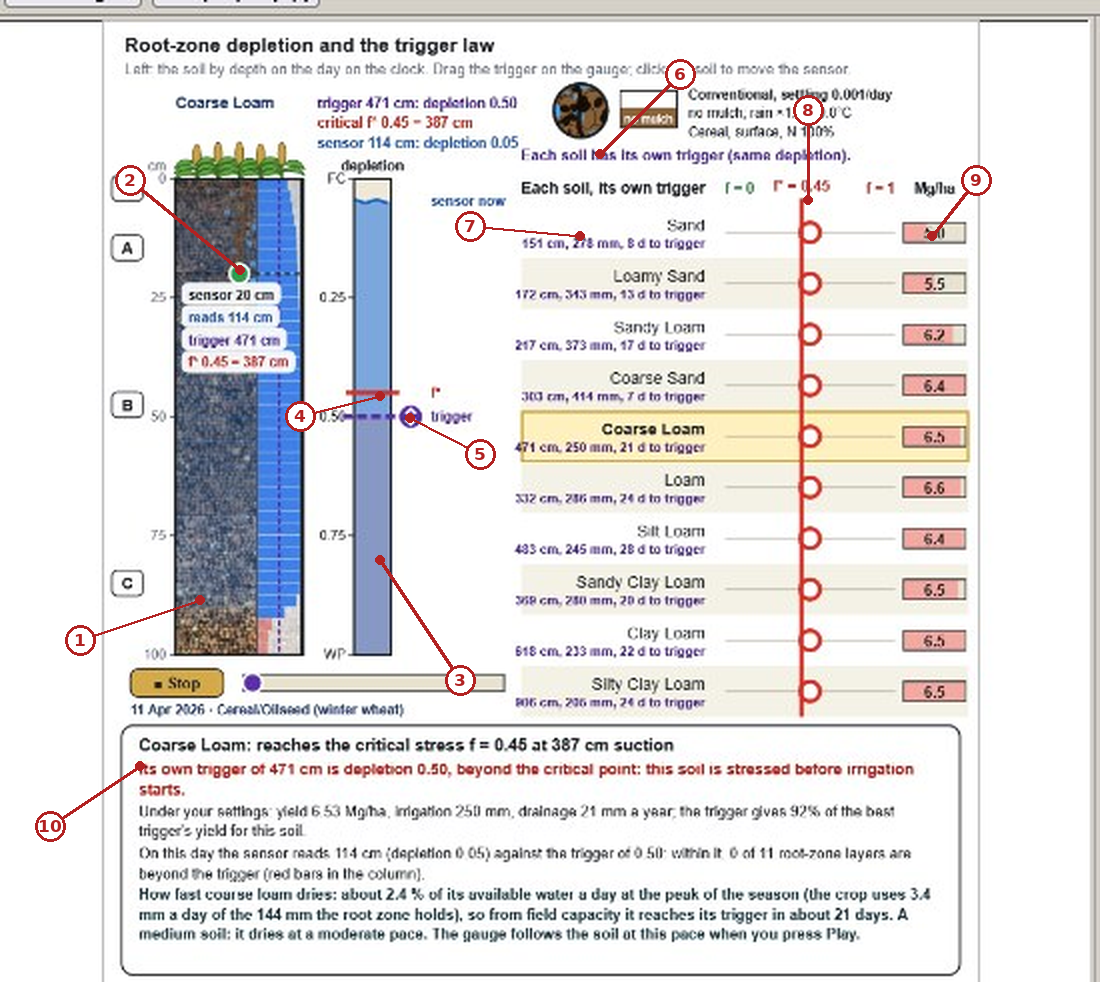
\includegraphics[width=\textwidth,height=0.42\textheight,keepaspectratio]{../figures/annot/p4_fig-soft_0.png}\end{center}

\textbf{What the numbered labels point to (picture 1 of 3: Trigger law layer: depletion, sensor and the trigger of every soil.).}
\begin{enumerate}[nosep,label=\protect\circled{\arabic*}]
\item The soil column of the chosen soil (coarse loam) from 0 to 100\,cm, coloured by its water content on the day shown; the roots are drawn to their depth.
\item The sensor at 20\,cm (green dot). Its box reads the suction of the day (114\,cm), the trigger (471\,cm) and the critical suction $h^*$ of $f^*=0.45$ (387\,cm) for this soil.
\item The depletion gauge: $f=0$ at field capacity (FC, top) to $f=1$ at the wilting point (WP, bottom). The blue fill is the water left on the day.
\item The red line $f^*$: the depletion beyond which the simulated yield falls by more than 5 \%; the same 0.45 for every soil.
\item The trigger (purple dot) at depletion 0.50. Dragging it moves the trigger; it sits below the red line, so this setting stresses the crop before irrigating.
\item Header of the right panel: each soil gets its own trigger for the same depletion, because the same depletion is reached at a different suction in every soil.
\item One soil row (sand): the suction at which this soil reaches the same depletion, the simulated irrigation of a year with that trigger and the days from field capacity to the trigger, ``151\,cm, 278\,mm, 8 d to trigger''.
\item The red column $f^*=0.45$; the circle on each row marks where the trigger of the left panel lies on that soil's depletion scale.
\item Yield boxes (Mg/ha): the simulated yield with that soil's trigger. Equal yields across soils are the point of soil-specific triggers.
\item The diagnosis in words: the trigger, the critical point, the season totals and how fast the soil dries (2.4 \% of its available water a day; trigger reached in about 21 days).
\end{enumerate}

\textbf{Equations behind this screen.} The numbers on the screen are computed as follows.
\begin{enumerate}[nosep,label=(\roman*)]
\item Depletion of a soil at suction $h$ (0 at field capacity, 1 at the wilting point): $f(h)=\dfrac{S_e(100)-S_e(h)}{S_e(100)-S_e(15\,849)}$, with $S_e(h)=[1+(\alpha h)^n]^{-(1-1/n)}$; 100\,cm is field capacity and 15\,849\,cm ($pF=4.2$) the wilting point.
\item Critical suction of a soil for the common depletion $f^*=0.45$: $S_e^*=S_e(100)-f^*[S_e(100)-S_e(15\,849)]$, then $h^*=\alpha^{-1}\bigl[(S_e^*)^{-1/m}-1\bigr]^{1/n}$, $m=1-1/n$. For coarse loam this gives 387\,cm, the number in the sensor box.
\item The trigger of a soil for depletion $f_t$ is found the same way with $f_t$ in place of $f^*$ (471\,cm for $f_t=0.50$); the program solves $f(h)=f_t$ by bisection on $\log_{10}h$.
\item Readily available water: $\mathrm{RAW}=f_t\cdot\mathrm{TAW}$, with $\mathrm{TAW}$ the available water of the root zone (144\,mm here).
\item Days from field capacity to the trigger: $t=f_t\,\mathrm{TAW}/ET_c$; for coarse loam $0.50\times144/3.4\approx21$\,days, as written in the diagnosis.
\item The reach of the article decides whether the trigger can ever be read: if $h_t>h_c$ (\cref{eq:s-hc}) the crop cannot dry the soil to the trigger and the trigger is blind.
\end{enumerate}

\begin{center}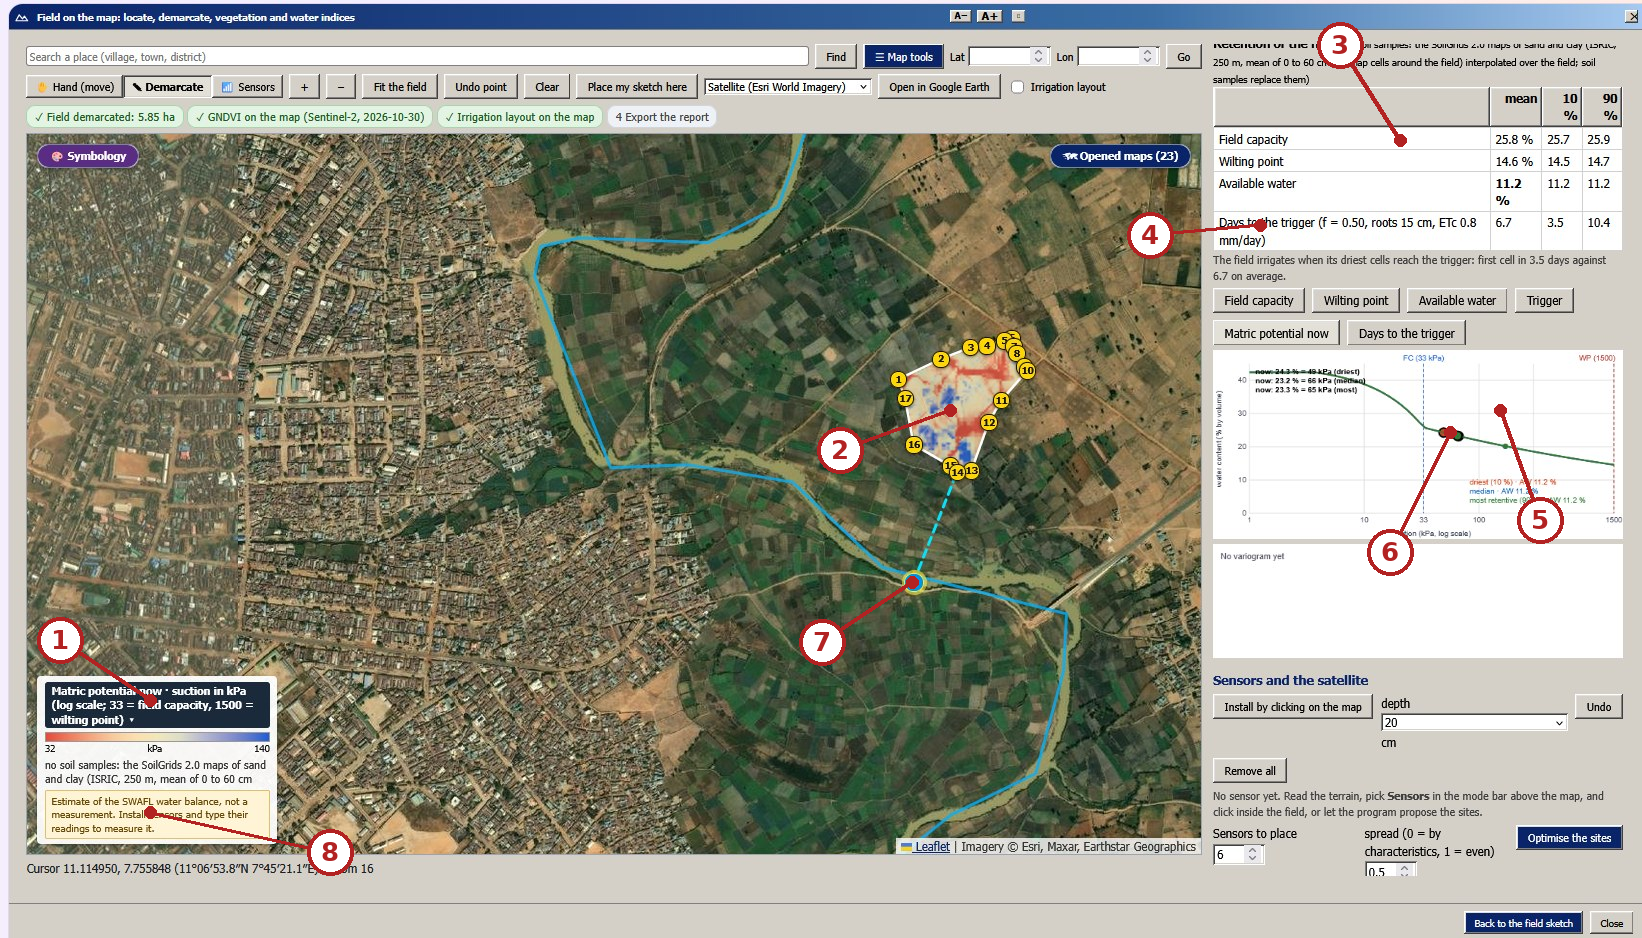
\includegraphics[width=\textwidth,height=0.42\textheight,keepaspectratio]{../figures/annot/p4_fig-soft_1.png}\end{center}

\textbf{What the numbered labels point to (picture 2 of 3: Matric potential on a 5.85\,ha field near Zaria, from mapped retention curves.).}
\begin{enumerate}[nosep,label=\protect\circled{\arabic*}]
\item Legend of the map: matric potential now as suction in kPa on a log scale (33\,kPa = field capacity, 1\,500\,kPa = wilting point); red is dry, blue is wet.
\item The field, divided into map cells; each cell has its own retention curve and its own water content now, so the suction varies within the field.
\item Retention of the field: field capacity, wilting point and available water, as the mean of the cells and the 10 \% and 90 \% cells.
\item Days to the trigger ($f=0.50$, roots 15\,cm, $ET_c=0.8$\,mm/day): 6.7 days on average, 3.5 for the driest cells.
\item The retention curves of the driest, median and most retentive cells: water content against suction (kPa, log scale), with field capacity and wilting point as vertical lines.
\item The state points: where each of the three cells is today on its curve (the ``now lines give the water content and suction).
\item The water source chosen for the field (river intake), joined to the field by the dashed line.
\item The note that the map is an estimate from the SWAFL water balance; sensors placed on the map replace the estimate by measurements.
\end{enumerate}

\textbf{Equations behind this screen.} The numbers on the screen are computed as follows.
\begin{enumerate}[nosep,label=(\roman*)]
\item Field capacity and wilting point of each cell from its sand $S$, clay $C$ and organic matter $OM$ (fractions, SoilGrids 2.0, 0--60\,cm) by the regressions of Saxton and Rawls (2006): $\theta_{33}$ and $\theta_{1500}$.
\item Slope of the retention curve: $\lambda=\dfrac{\ln1500-\ln33}{\ln\theta_{33}-\ln\theta_{1500}}$; for $\psi\ge33$\,kPa, $\theta(\psi)=\theta_{33}\,(\psi/33)^{-\lambda}$.
\item Available water $AW=\theta_{33}-\theta_{1500}$, and the trigger water content $\theta_t=\theta_{33}-f\,(\theta_{33}-\theta_{1500})$.
\item Matric potential now, the inverse of the curve: $\psi=33\,(\theta/\theta_{33})^{-1/\lambda}$\,kPa, with $\theta$ the water content of the cell from the water balance (or from sensors when installed).
\item Days to the trigger: $t=\max\bigl(0,\,(\theta-\theta_t)\,z_r\cdot10/ET_c\bigr)$ with $z_r$ in cm and $ET_c$ in mm/day. With $AW=0.112$, $f=0.5$, $z_r=15$\,cm, $ET_c=0.8$: at field capacity $t=0.5\times0.112\times150/0.8=10.5$\,days; the mean 6.7 days is shorter because the cells are already below field capacity.
\item Units: 1\,kPa $\approx$ 10.2\,cm of water, so 33\,kPa $\approx$ 337\,cm and 1\,500\,kPa $\approx$ 15\,300\,cm, the same limits as the suction scale of the article.
\end{enumerate}

\begin{center}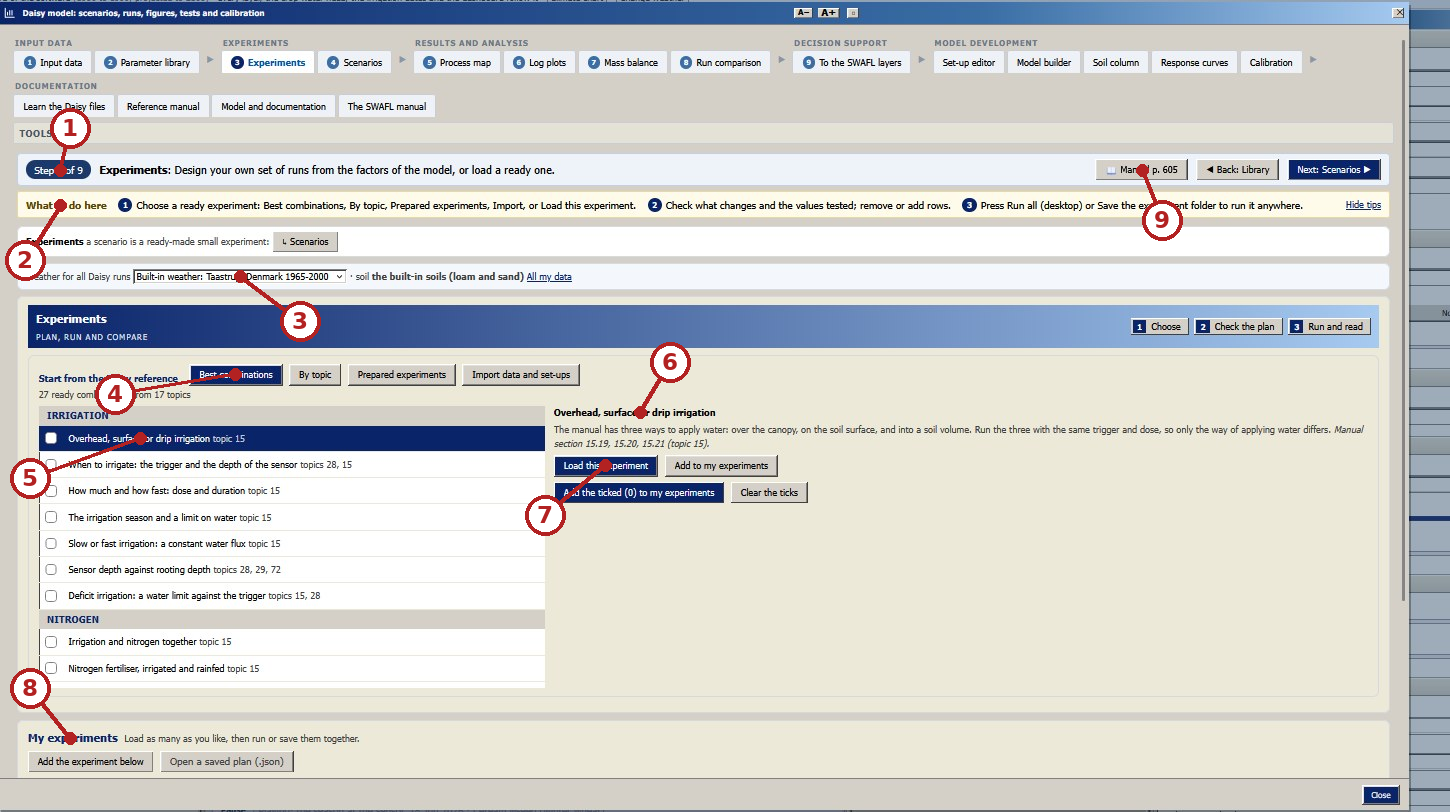
\includegraphics[width=\textwidth,height=0.42\textheight,keepaspectratio]{../figures/annot/p4_fig-soft_2.png}\end{center}

\textbf{What the numbered labels point to (picture 3 of 3: Daisy workbench, step 3 of 9: ready-made experiments (trigger and sensor depth, dose, method) and the user's own.).}
\begin{enumerate}[nosep,label=\protect\circled{\arabic*}]
\item Step 3 of 9 of the work flow: experiments, between the parameter library (step 2) and the scenarios (step 4).
\item What to do here: choose a ready experiment, check the factors and levels, then run all or save the folder.
\item The weather and soils of every run of the experiment (built-in weather Taastrup, Denmark).
\item Best combinations: 27 ready experiments from 17 topics of the Daisy reference manual.
\item One ready experiment, ``Overhead, surface or drip irrigation'', the comparison of methods used in the article.
\item Its description: the three methods are run with the same trigger and dose, so only the way of applying water differs.
\item Load this experiment: puts its factors and levels in the plan, where rows can be removed or added.
\item My experiments: several loaded experiments are run or saved together.
\item Link to the page of the Daisy manual that documents these settings (p.\,605).
\end{enumerate}

\textbf{Equations behind this screen.} The numbers on the screen are computed as follows.
\begin{enumerate}[nosep,label=(\roman*)]
\item Number of Daisy runs of an experiment with factors of $n_1,n_2,\dots$ levels and a budget $B$: $N=\min\bigl(\prod_i n_i,\,B\bigr)$.
\item If $\prod_in_i>B$, a Latin hypercube of $B$ runs is drawn so that each level of factor $i$ is used $\lfloor N/n_i\rfloor$ or $\lceil N/n_i\rceil$ times.
\item Every run is one full Daisy simulation; its annual fluxes (transpiration, soil evaporation, drainage, irrigation, yield) are what the article compares between methods with the rainfed twin, $\eta_X=\sum(X-X_0)/\sum I$.
\end{enumerate}

\textbf{What it shows.} The analysis in SWAFL Desktop 1.1.0 (real screenshots of the release). Panels: (a) Trigger law layer: depletion, sensor and the trigger of every soil. (b) Matric potential on a 5.85\,ha field near Zaria, from mapped retention curves. (c) Daisy workbench, step 3 of 9: ready-made experiments (trigger and sensor depth, dose, method) and the user's own.

\textbf{How to read the labels, symbols and colours.} (a) The trigger-law layer: on the left the soil column with the sensor (dot) and the depletion bar; on the right one row per soil with its own trigger (red marks), the yield (boxes) and a gauge of the season. (b) The matric potential of the Zaria field, cell by cell; the colour bar is in kPa (33 = field capacity, 1500 = wilting point). (c) The ready-made experiments of the Daisy workbench.

\textbf{What affects it, and why it happens.} The trigger law shows each soil's own trigger because each soil reaches the same depletion at a different suction; the suction map varies with the soil texture mapped from SoilGrids; the workbench runs new experiments on any soil. These are screens of the software, not results; they show where a user finds the reach and the triggers of each soil, how the suction varies over a real field (with the soil texture from SoilGrids), and how new trigger, dose and method experiments are run.

\textbf{How it is made.} Screen capture of SWAFL Desktop 1.1.0 (not regenerated).

